\documentclass[fleqn,10pt]{wlscirep}
\usepackage[utf8]{inputenc}
\usepackage[T1]{fontenc}

\usepackage{amsthm}	% per la stilizzazione dei teoremi e per gestire extra simboli matematici, size, space, font, etc..
\usepackage{amsopn}	% per stilizzazione di alcuni operatori matematici (e.g. lim e log)
\usepackage{amscd}	% per gestire frecce e circolarità tramite frecce su più livelli in un'equazione (tipo grafi)
\usepackage{amssymb} % per i simboli matematici
\usepackage{array}	% per creare e gestire array
\usepackage{actuarialsymbol} % per simboli attuariali e di matematica finanziaria 
\usepackage{mathtools} % per integrare amsmath
\usepackage{makeidx} % per l'indice 
\usepackage{multicol} % per gesttire più colonne nelle tabelle 
\usepackage{multirow} % per gestire più righe nelle tabelle
\usepackage{caption} % per gestire legende e descrizioni di tabelle, grafici e figure
\usepackage{float} % per gestire posizinamento grafici, tabelle e figure varie
\usepackage{enumerate} % pacchetto per le liste numerate 
\usepackage{graphicx} % pacchetto base per inserire i grafici  
\usepackage{subfig} % gestione di figure allineate
\usepackage{booktabs} % per l'ottimizzazione delle tabelle
\usepackage{lineno}
\linenumbers

\title{Enhancing diagnostic of stochastic mortality models leveraging contrast trees. An application on Italian data}

\author[1]{Susanna Levantesi}
\author[1]{Matteo Lizzi}
\author[2*]{Andrea Nigri}

\affil[1]{Department of Statistics, Sapienza University of Rome, Viale Regina Elena 295-G, 00161 Rome, Italy}
\affil[2]{Department of Economics, Management and Territory, University of Foggia, Foggia, Italy} 
\affil[*]{andrea.nigri@unifg.it}

%\keywords{Keyword1, Keyword2, Keyword3}

\begin{abstract}
%%%%%%%%%%%%%%%%%%%%%%%%%%%%%%
%\textit{The abstract should be no more than 200 words; Abstract must not include subheadings or citations.}\\
%%%%%%%%%%%%%%%%%%%%%%%%%%%%%%
The rise in longevity in the twentieth century has led to a growing interest in modeling mortality, and new advanced techniques such as machine learning have recently joined to more traditional models, such as the Lee-Carter or the Age Period Cohort. 
However, the performances of these models, in terms of fitting to the observed data, are difficult to compare in a unified framework.
The goodness-of-fit measures summarizing the discrepancy between the estimates from the model and the observed values are different for traditional mortality models and machine learning. We, therefore, employ a new technique, Contrast trees, which, leveraging on decision trees, provides a general approach for evaluating the quality of fit of different kinds of models by detecting the regions in the input space where models work poorly. 
Once the low-performance regions are detected, we use Contrast boosting to improve the inaccuracies of mortality estimates provided by each model. 
To verify the ability of this approach, we consider both standard stochastic mortality models and machine learning algorithms in the estimate of the Italian mortality rates from the Human Mortality Database. 
The results are discussed using both graphical and numerical tools, with particular attention to the high-error regions. 
\end{abstract}

\begin{document}

\flushbottom
\maketitle
% * <john.hammersley@gmail.com> 2015-02-09T12:07:31.197Z:
%
%  Click the title above to edit the author information and abstract
%
\thispagestyle{empty}

%%%%%%%%%%%%%%%%%%%%%%%%%%%%%%
%\noindent \textit{Please note: Abbreviations should be introduced at the first mention in the main text – no abbreviations lists. Suggested structure of main text (not enforced) is provided below. The main text should be no more than 4,500 words (not including Abstract, Methods, References and figure legends). Articles should ideally be no more than 11 typeset pages.}
%%%%%%%%%%%%%%%%%%%%%%%%%%%%%%

\section*{Introduction}
%%%%%%%%%%%%%%%%%%%%%%%%%%%%%%
%\textit{The Introduction section expands on the background of the work (some overlap with the Abstract is acceptable). The introduction should not include subheadings.}\\
%%%%%%%%%%%%%%%%%%%%%%%%%%%%%%

%The life expectancy rise that has occurred in the last decades constitutes a great conquest but contemporarily creates substantial challenges for life insurers and social security schemes providing benefits related to illness, or survival of people. Important policy decisions are based on the human longevity reliable estimates, and public pension policies are a prime example. Thereby, understanding longevity dynamics over age and time is crucial, as they are one of the driving forces of population change. 
Since 1980, innovative approaches and developments in mortality modeling have been constantly proposed. 
Mortality analysis has received a considerable contribution from statistical science, building solid foundations for the evolution of mortality methods. Estimating longevity is not straightforward; accuracy depends on the particular situation or trends, and it is not easy to comprehend when a method will good perform. Indeed, new mortality models will appear in the literature but may take years before they can be fully evaluated. As stated by \cite{Booth}, the accuracy of mortality estimates should be regularly tested to set the improvement evidence. Researchers appear to be more focused on technical progress of a method rather than on the accuracy of the estimation provided, focusing on minimizing the bias.

Several approaches have been used to model the mortality surface, determining how death rates change over time. Until the 1980s, mortality models were relatively simple and involved a fair degree of subjective judgment (see \cite{Pollard} for a detailed review on this aspect). The growing availability of reliable data, in lockstep with the improvement of statistical-mathematical methods, has allowed the creation of ever-finer mortality models. According to \cite{Booth}, literature would suggest three approaches to demographic modeling. 
The first one (explanation) makes use of structural or epidemiological models from certain causes of death. A classic example is the dependence of lung cancer on tobacco smoking. The second one (expectation) is based on subjective expert opinion, involving varying degrees of formality. Finally, the third and most commonly used approach is extrapolative, using the regularity typically found in age patterns and trends over time.
This approach includes the more complex stochastic mortality models such as the Lee-Carter \cite{LC92} and, more generally, the Generalized Age Period Cohort (GAPC) model. Despite the Lee-Carter model being widely recognized as the cornerstone of mortality modeling and forecasting, over the last decade, scholars suggested additional approaches that also gained interest in the academic world \cite{BDV2002,RH,CBD06,CBD09}.

Despite models like the Lee-Carter and its variants having been widely used, becoming a benchmark for many newly proposed methodologies, they present several shortfalls. In this line, \cite{CBD08} tried to address the issue of what would be the best way to estimate mortality, exhibiting interesting criteria that a good mortality model should hold. They referred to good-practice guidelines such as the consistency with historical data and the long-term dynamics, biologically reasonable. Following this line of research, recent longevity literature stimulated the use of machine learning techniques in demographic research allowing the integration of stochastic models into a data-driven approach. 

The significant reduction in the forecasting error reached by the application of machine learning techniques became particularly useful for both researchers and practitioners. The main contributions are from \cite{Deprez,LevPiz,LevNi}. The common idea behind all these works is to improve the fitting accuracy of canonical models using machine learning algorithms. In other words, to correct the mortality surface produced by standard stochastic mortality models. All of the proposed methods calibrate a machine learning estimator used to adjust (and improve) mortality rates estimated by the original mortality model. Those authors show that mortality modeling can benefit from machine learning as it better captures patterns that traditional models do not identify. 

The need for new tools for comparing models' performances is evident to understand mortality evolution more accurately. 
This paper contributes to the literature on mortality modeling by introducing an innovative approach based on machine learning techniques that demographers have not yet explored, contributing to the undervalued field of model assessment. 
\color{blue}
This approach, namely Contrast trees, recently proposed by \cite{Friedman2020}, and here applied to mortality data, helps evaluate the accuracy of the mortality estimates (fitted mortality rates) given by models that are not treatable with model selection criteria based on the likelihood function. Therefore, this technique provides a unified framework for assessing and comparing the goodness-of-fit to historical data of traditional mortality models with machine learning algorithms.
Our paper highlights the ability of Contrast trees to identify the regions in the predictor variables space that show very high values of the error rate quantified by a discrepancy measure. The regions’ width and shape change from model to model. \color{black}
Moreover, in addition to evaluating the accuracy of the models, the Contrast trees enables improving the performance of the models through a boosting procedure that reduces the inaccuracies. We use this methodology, namely Contrast boosting, to improve \color{blue}the fitting of historical mortality data.
According to the demographic literature, the reliable estimation of mortality data may refer not only to the extrapolation but also to an accurate fitting of the historical mortality surface. For instance, in longevity analysis is common to deal with subpopulations i.e. regions or provinces, characterized by a high level of stochasticity often due to a small number of count data at single ages. This is the case in which specific ages or years are not covered with data information, making the mortality estimation challenging. Our approach is crucial to evaluate the mortality matrix estimation provided by a mortality model and to ensure estimation effectiveness by comparing different methods.
To summarize, through this new technique based on Contrast trees, we aim to find the best model that fits observed mortality rates by grasping and detecting the inaccuracies of any model and boosting its predictive power. \color{black}

The remainder of this paper is organized as follows: Section 2 introduces the model framework, both Contrast trees and Contrast boosting. 
In Section 3, we describe the numerical implementation, also providing an overview of the mortality models, expressed in a regression framework, which we assess by the Contrast trees approach. We devote a specific sub-section to explanation and discussion of the numerical results. 
Section 4 concludes the paper, providing other possible practical implementations of the method in mortality assessment and the limitations of our research.

%-------------------------------------------------------------
\section*{Materials and Methods}
%-------------------------------------------------------------
%\textit{Topical subheadings are allowed. Authors must ensure that their Methods section includes adequate experimental and characterization data necessary for others in the field to reproduce their work.}

\subsection*{Data source}

We consider the Italian mortality data available in the Human Mortality Database (HMD) over the period 1950-2018. We refer to the male population aged \color{blue}0-90, analyzing the age groups 0-29, 30-60, and 61-90 separately to provide further evidence of the differences in mortality that characterizes the younger ages, the adult ages, and the older ages. 
We split the data set into a training set and a test set according to the common splitting rule 70\%-30\%. 
We use the training set to obtain the parameters' estimate of each model. We apply the parameters' estimate in the test set to evaluate the out-of-sample performance. Finally, we will calculate the out-of-sample errors using data from the test set.
\color{black}
The dataset partition is obtained by using the dissimilarity-based compound selection proposed in \cite{Willett1999}.

\subsection*{Mortality rate}
We calculate the central death rates $m_{x,t}$ for each age $x$ and year $t$ according to the following formula:
\begin{equation} 
\label{eq:mxt}
m_{x,t}=\frac{D_{x,t}}{E_{x,t}}
\end{equation}
Where $D_{x,t}$ is the number of deaths aged $x$ in year $t$, and $E_{x,t}$ are the exposures-to-risk aged $x$ in year $t$.

\subsection*{Mortality models}
\color{blue}In the following, we briefly describe the four models to which the Contrast trees methodology is applied. The scope is to evaluate the models' quality of fit. \color{black}
The first two models belong to the family of generalized age-period-cohort (GAPC) that are expressed in a regression framework to be suitable for applying Contrast trees, which requires data organized in columns. The last two are well-known machine learning techniques also used for regression tasks.\\

\subsubsection*{Lee-Carter (LC) model}
The original LC model\cite{LC92} assumes that:
\begin{equation} 
\label{eq:LC}
\log{\left(m_{x,t}\right)}=\alpha_{x}+\beta_{x} \kappa_{t}
\end{equation}
The age-specific parameter $\alpha_x$ provides the average age profile of mortality, the age-period term $\beta_{x}\cdot\kappa_t$ describes the mortality trends, with $\kappa_t$ the time index and $\beta_{x}$ modifying the effect of $\kappa_t$ across ages. The model is subject to the following constraints on $\kappa_t$ and $\beta_x$: $\sum_{t}{\kappa_t}=0$ and $\sum_{x}{\beta_x}=1$.
%Future mortality rates are obtained by modeling the time index $\kappa_{t}$ through an autoregressive integrated moving average (ARIMA) process. In general, a random walk with drift properly fits the data. \\
%\begin{equation} 
%\kappa_{t} = \kappa_{t-1} + \delta + \epsilon_t, \quad \epsilon_t \sim N(0, \sigma^{2}_k)
%\end{equation}
%where $\delta$ is the drift parameter and $\epsilon_t$ are the error terms, normally distributed with null mean and variance $\sigma^{2}_k$.
\color{blue}The LC model can be reformulated into a Generalized Non-linear Model (GNM) framework, as in \cite{Villegas2018}, following the approach proposed by \cite{BDV2002}, which assume that deaths are independent Poisson distributed. The authors use a GNM and apply the maximum likelihood method to fit the model to historical data. Under this specification, the LC model can be seen as a non-linear regression model where mortality rates are the target variable, predicted using features (age and time) \cite{RichmanWuthrich}. \color{black}

\subsubsection*{Age-Period-Cohort (APC)}
We use the model's version reformulated into a Generalized Linear Models (GLM) framework \cite{Alai2014}:
\begin{equation} 
\label{eq:APC}
\color{blue} \log{\left(m_{x,t}\right)}=\beta_{0} +\beta_{1,x}+\beta_{2,t} +\beta_{3,t-x}
\end{equation}
Where the regression coefficients $\beta_{1,x}$, $\beta_{2,t}$, \color{blue}$\beta_{3,t-x}$ \color{black} are the age trend, the period trend and the cohort trend \color{blue}($t-x$ represents the year of birth)\color{black}.

\subsubsection*{Gradient Boosting Machine (GBM)}
GBM is a tree-based algorithm proposed by \cite{Friedman} that uses fixed-size decision trees as weak learners. The prediction is obtained by a sequential approach, where each decision tree uses the information from the previous one to improve the current fit. Given a current model fit, $F_{m}(\mathbf{x})$, the algorithm provides a new estimate, $F_{m+1}(\mathbf{x})=F_{m}(\mathbf{x})+ h_m(\mathbf{x})$, where $h_m(\mathbf{x})$ is the weak learner fitted on the model residuals $y-F_{m}(\mathbf{x})$ with $y$ target variable.

\subsubsection*{eXtreme Gradient Boosting Machine (XGBM)}
XGBM is an efficient implementation of gradient boosting decision trees proposed by \cite{Chen}, and designed to be fast to execute and highly effective. To verify if a simple data preprocessing has some meaningful effect on the quality of models, we apply XGBM to both raw and preprocessed data: the latter is obtained by centering and scaling the raw data using mean and standard deviation.

\color{blue}
\subsection*{Traditional diagnostic tools}
In the following, we briefly mention some traditional diagnostic tools that are often used in the literature to assess the goodness-of-fit of a mortality model. 
\begin{itemize}
\item Analysis of mortality residuals (or standardized mortality residuals) calculated as the difference between the crude estimate of mortality rate by age and year based on observed data and the corresponding estimated mortality rate using a specified mortality model. For example, \cite{Cairns2010} verified that they are consistent with the hypothesis of i.i.d. $N(0,1)$ and have zero correlation both across adjacent ages and across adjacent years.
\item Proportion of variance explained ($R^2$) by the model or the parameters of the model (see, e.g., \cite{Bongaarts2005})
\item Model selection criteria that penalize the log-likelihood with the increase in number of parameters: Akaike Information Criterion (AIC), Schwarz-Bayes Criterion (SBC) (or Bayes Information Criterion (BIC)) and Likelihood-ratio test (LRT) \cite{Li2009}. Note that in this case the evaluation of the goodness-of-fit is given on the basis of the log-likelihood. 
\item Qualitative model selection criteria: \cite{CBD08} provide a list of criteria that might be considered desirable in a mortality model, such as, e.g., ease of implementation, parsimony, and transparency. Relating to the fitting ability to the observed data, the model should be consistent with historical data, and parameter estimates should be robust relative to the range of data used. For example, \cite{Djeundje2022} consider consistency, stability, and parsimony in addition to standard goodness-of-fit indices (deviance residual, BIC, and residual patterns).
\item Checking for the absence of autocorrelation in the residuals of the model by the Portmanteau test (see, e.g., \cite{Torri2011}).
\end{itemize}
\color{black}

\subsection*{Contrast trees}
\color{blue}Contrast trees is an innovative approach that, leveraging tree-based machine learning techniques, allows for deeply assessing the goodness-of-fit of a model by identifying where the model performs worse. \color{black}
Specifically, the goal of the Contrast trees method is to uncover regions in the predictor variables space presenting very high values of the error rate quantified by a discrepancy measure \cite{Friedman2020}. \color{blue}In the context of mortality modeling, the main feature that distinguishes this method from the traditional diagnostic methods mentioned above is the ability to automatically identify the regions in which a given model provides a high error for certain combinations of ages and calendar years.
Furthermore, Contrast trees have the advantage of being easy to interpret and can be used as a diagnostic tool to detect the inaccuracies of every kind of model, for example, both those whose parameters estimate is based on a likelihood function and those based on machine learning algorithms. Our analysis shows how Contrast trees can be used for assessing the goodness-of-fit of different mortality models to observed data. 
\color{black}

Suppose to have a set of predictor variables $x = (x_1, x_2,...,x_p)$ and two outcome variables $y$ and $z$ for each $x$. We aim to find those values of $x$ for which the respective distributions of $y | x$ and $z | x$, or some statistics such as mean or quantiles, are most different. In summary, Contrast trees provide a lack-of-fit measure for the conditional distribution $p_y(y | x)$, or some statistics.\\
Consider the $M^{th}$ iteration, where the tree splits the space of the predictor variables into $M$ disjoint regions $\lbrace R_m\rbrace^M_{m=1}$, each one containing a subset of the data. We denote $f_m^{(l)}$ and $f_m^{(r)}$ the fraction of observations in the left and right region with respect to $R_m$, respectively. While, the quantities $d_m^{(l)}$, $d_m^{(r)}$ respectively represent the discrepancy measures associated to the fractions $f_m^{(l)}$ and $f_m^{(r)}$. Given a specified subset of the data $\lbrace x_i,y_i,z_i \rbrace_{x_i\in R_m}$, a discrepancy measure between $y$ and $z$ values can be generally defined as:
\begin{equation}
\label{eq:dm}
d_m=D\left( \lbrace y_i\rbrace_{x_i\in R_m},\lbrace z_i\rbrace_{x_i\in R_m}\right)
\end{equation}
The quality of a split is quantified by the following measure:
\begin{equation}
Q_m(l,r)=\left(f_m^{(l)} \cdot f_m^{(r)}\right) \cdot max\left(d_m^{(l)}, d_m^{(r)} \right)^{\beta}
\end{equation}
The factor $\left(f_m^{(l)} \cdot f_m^{(r)}\right)$ discourages highly asymmetric splits in anticipation of further splitting, while the other factor $max\left(d_m^{(l)}, d_m^{(r)} \right)^{\beta}$ attempts to isolate the $R_m^{(l)}$ and $R_m^{(m)}$ regions with high discrepancy. The parameter $\beta$ regulates the relative influence of the two factors but, as stated by \cite{Friedman2020}, results are insensitive to its value. We will use $\beta=2$ in our analysis.

The choice of the discrepancy measure depends on the problem to be solved, allowing Contrast trees to be applied to a variety of problems \cite{Friedman2020}. They are similar to loss criteria in prediction problems. The discrepancy measures that could be appropriate to represent the problem under investigation are the following:
\begin{equation}
\label{eq:dm1}
d_m^{[1]} = \frac{1}{N_m} \sum_{x_i \in R_m} \lvert y_i-z_i \rvert
\end{equation}
%
\begin{equation}
\label{eq:dm2}
d_m^{[2]} = \frac{1}{2N_m-1} \sum_{i =1}^{2N_m-1} \frac{\left| \hat{F}_y(t_{(i)})-\hat{F}_z(t_{(i)})\right|}{\sqrt{i\cdot(2N_m-i)}}
\end{equation}
where $N_m$ is the number of observations in the region $R_m$,  $t_{(i)}$ is the $i^{th}$ value of $t$ in sorted order, and $\hat{F}_y$ and $\hat{F}_z$ are the respective empirical cumulative distributions of $y$ and $z$. See \cite{Friedman2020} for further details about the tree split procedure.\\
In numerical applications, for sake of simplicity, we use the discrepancy measure $d_m^{[1]}$.

\subsubsection*{Lack-of-fit contrast curves}

The results obtained by applying the Contrast trees to different models can be summarized in the lack-of-fit contrast curves, which have point coordinates 
$$[f_m,\bar{d}_m]$$
where $f_m=\frac{1}{N}\sum_{d_j\geq d_m}N_j$ is the fraction of observations in the region $R_m$ containing $N_m$ observations, and $\bar{d}_m=\frac{\sum_{d_j\geq d_m}d_j N_j}{\sum_{d_j\geq d_m}N_j}$ is the average discrepancy.

From the above expressions, we can deduce that the lack-of-fit curves by construction are decreasing. By way of example, we show a typical pattern of this curve in Fig. \ref{fig:lof-ex}, where the leftmost point on the abscissa-axis provides the fractions of observations that fall into the regions with the higher discrepancy, while the rightmost point corresponds to all the observations ($f_m=1$).
Looking at the ordinate-axis, the leftmost point on each curve represents the $\bar{d}_m$ value of the largest discrepancy region of its corresponding tree; the rightmost point provides the $\bar{d}_m$ value across all regions. Points in between give a $\bar{d}_m$ value over the regions with the highest discrepancy that contain the corresponding fraction of observations \cite{Friedman2020}.
\begin{figure}[ht]
\centering
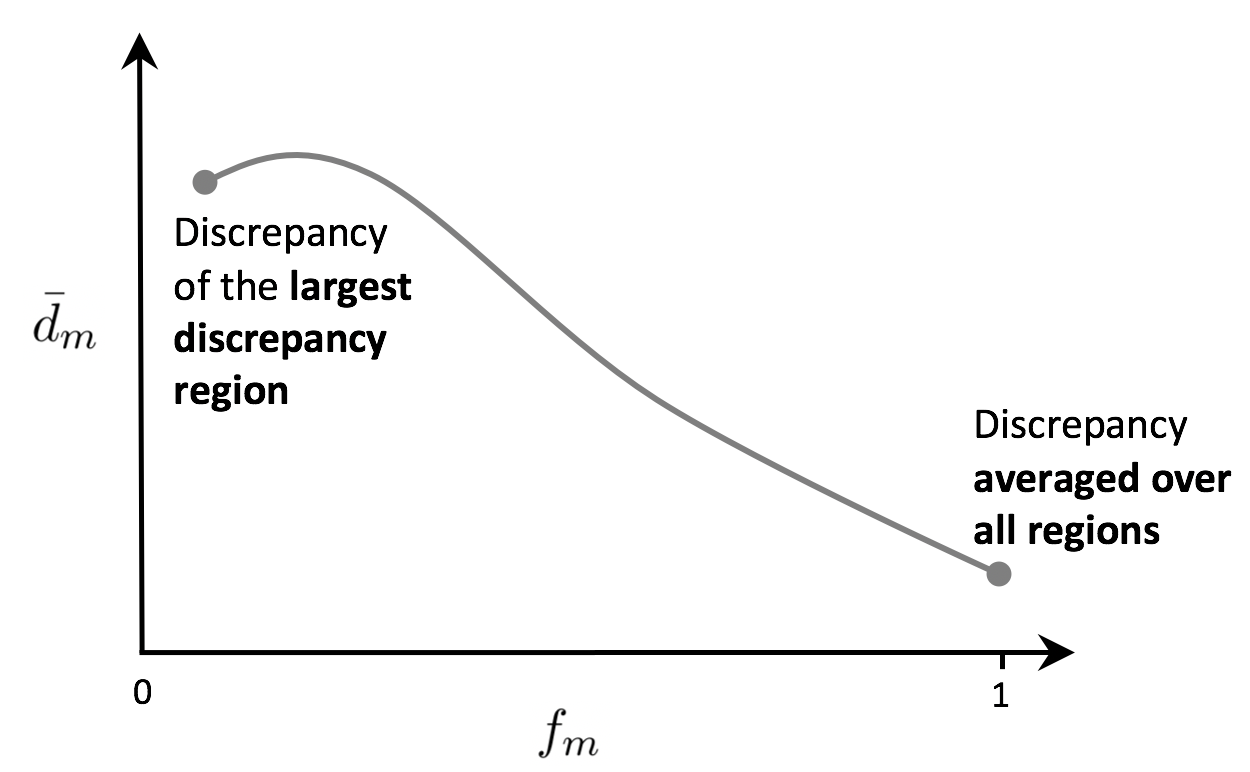
\includegraphics[width=0.45\textwidth]{lof_example.png}
\caption{Example of a lack-of-fit contrast curve}
\label{fig:lof-ex}
\end{figure}

\subsection*{Contrast boosting}

To improve the models accuracy, \cite{Friedman2020} proposes a contrast-boosting strategy that, dealing with the uncovered errors, can enable the regression models to provide more accurate predictions. Contrast boosting works by gradually modifying a starting value of $z$ to reducing its discrepancy with $y$ over the data. The resulting prediction is then affected by these modifications on the initial value of $z$.
We consider the estimation Contrast boosting, which takes $z$ as an estimate of a parameter of the full conditional distribution of a target variable given a set of predictor variables, $p_y(y | x)$.
The procedure consists of modifying the $z$ values within a certain region $R_m^{(1)}$ of a CT, so that its discrepancy with $y$ is zero, i.e. to set $d_m=0$ in Eq. \ref{eq:dm}.
This is an iterative procedure, where the first modification is from $z$ to $z^{(1)}=z+\delta^{(1)}_m$ for $x\in R^{(1)}_m$, the second from $z^{(1)}$ to $z^{(2)}=z+\delta^{(2)}_m$ for $x\in R^{(2)}_m$, and so on.
The $z$ values final estimate is then $\tilde{z}(x)=z(x)+\sum_{k=1}^{K}\delta_{m}^{(k)}$, where $K$ are the maximum number of iterations. In practice, each updated value of $z$ is contrasted with $y$ producing new regions $R^{(k)}_m$ ($1\leq k\leq K$) with corresponding updates $\delta_{m}^{(k)}$.

%-------------------------------------------------------------
\section*{Results}
%-------------------------------------------------------------
%\textit{Up to three levels of \textbf{subheading} are permitted. Subheadings should not be numbered.}\\

We implement the analyses using the \textit{conTree} R package developed by \cite{FriedmanNarasimhan2020}.
We set to 100 the maximum tree size corresponding to the number of regions. It is worth noting that the choice of this parameter is not straightforward because it involves a trade-off between discrepancy and interpretability. The smaller the trees, the larger the regions (defined by simple rules and easy to be interpreted). The larger the trees, the higher the potential to uncover small high discrepancy regions (defined by complex rules).
%Pruning strategies analogous to those in classification and regression trees based on cross-validation can also be employed to guide choice of tree size.

\color{blue} The models' performance results on the test set are summarized in the lack-of-fit contrast curves, deduced by contrasting the observed mortality data to the estimates provided by each model. These curves are shown in Fig. \ref{fig:lof} for the three different ages groups analyzed. The panels (a)-(c) of these figures refer to the lack-of-fit curves obtained without applying the Contrast boosting (Base models), while panels (d)-(f) refer to the lack-of-fit curves obtained after applying Contrast boosting to the output of the models (Boosted models).
For the 0-29 age group (Fig. \ref{fig:lof}, panel (a) and (d)), both APC and XGBM model have the lowest discrepancy values for each fraction of observations, providing the best fitting. The average discrepancy for this age group is higher than for the 30-60 age group. The 0-29 age group is known to be characterized by high accidental mortality, the so-called “accident hump” around age 20-25, due to accidental deaths or suicides caused by increased risk-taking behavior. Mortality at age 0-29 is therefore hard to predict, and Contrast boosting is not able to actually reduce the average discrepancy. \color{black}
For the 30-60 age group (Fig. \ref{fig:lof}, panel (b) and (e)), the APC model seems to best perform across all regions since the discrepancy values are consistently lower than those of the other models. For the XGBM models, we can observe that the model applied to preprocessed data (XGBM prep) performs better in the regions with the highest average discrepancy with respect to the model applied to raw data. From the scale of the plots, we can see that Contrast boosting reduces discrepancy across almost all regions for the GBM and LC models, where the relative effect of boosting is particularly evident. 
For the 61-90 age group (Fig. \ref{fig:lof}, panel (c) and (f)), the GBM model seems by far the worst performing model. 
Albeit the application of Contrast boosting significantly reduces the discrepancy, the GBM continues to be less accurate than the other models. It should also be noted that the effect of Contrast boosting in high-discrepancy regions for the other models is negligible, except for the APC.
\begin{figure}[ht]
\centering
\subfloat[Base model - Age 0-29]
{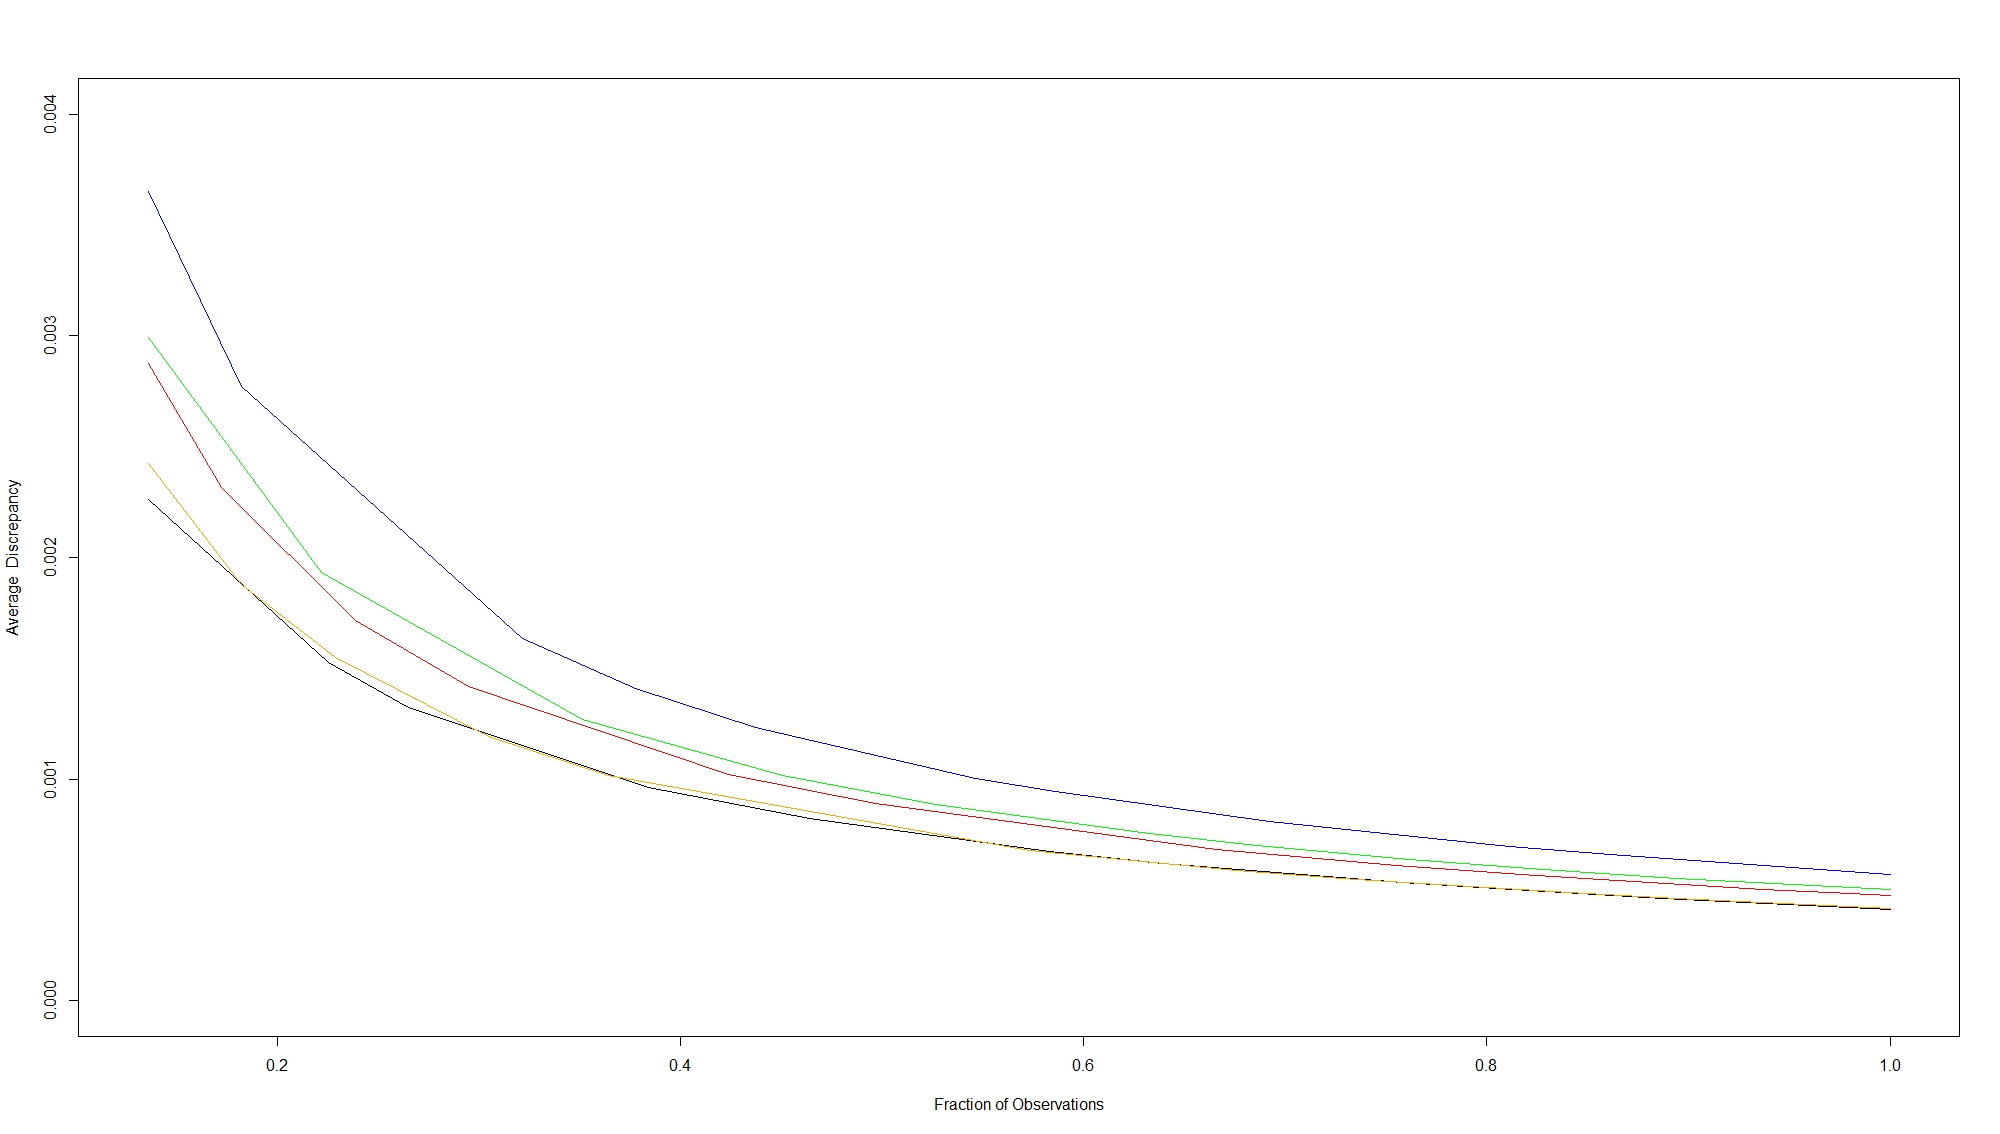
\includegraphics[width=0.31\textwidth]{lof_0}}\quad
\subfloat[Base model - Age 30-60]
{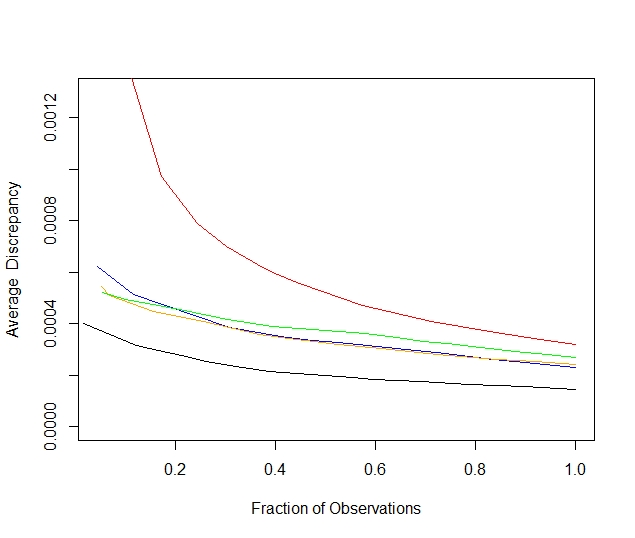
\includegraphics[width=0.31\textwidth]{lof}}\quad
\subfloat[Base model - Age 61-90]
{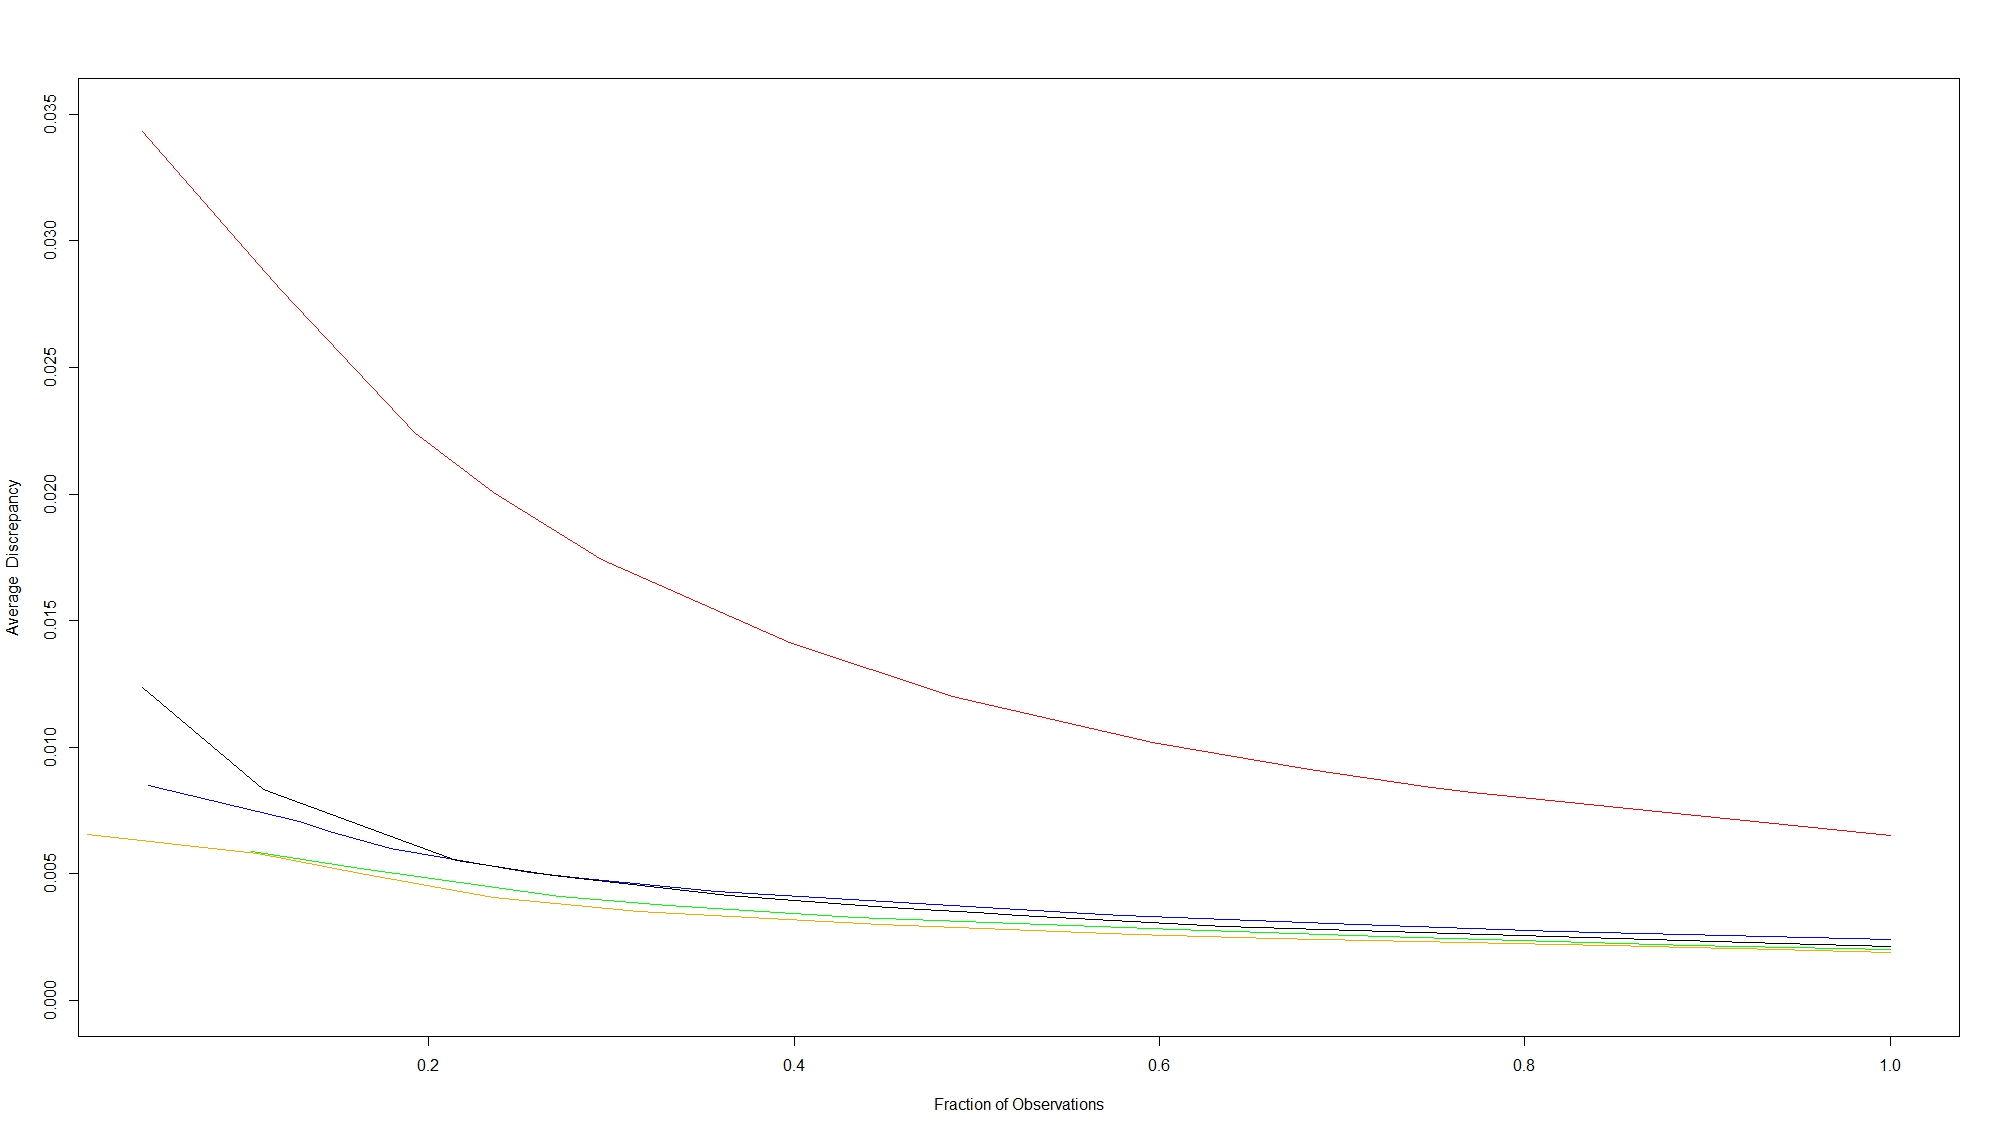
\includegraphics[width=0.31\textwidth]{lof_61}}\\
\subfloat[Boosted model - Age 0-29]
{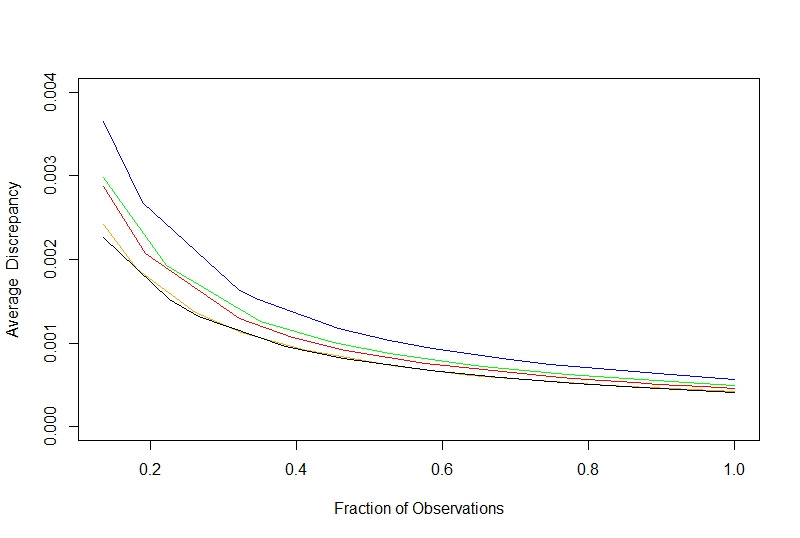
\includegraphics[width=0.31\textwidth]{lof_0_b}}\quad
\subfloat[Boosted model - Age 30-60]
{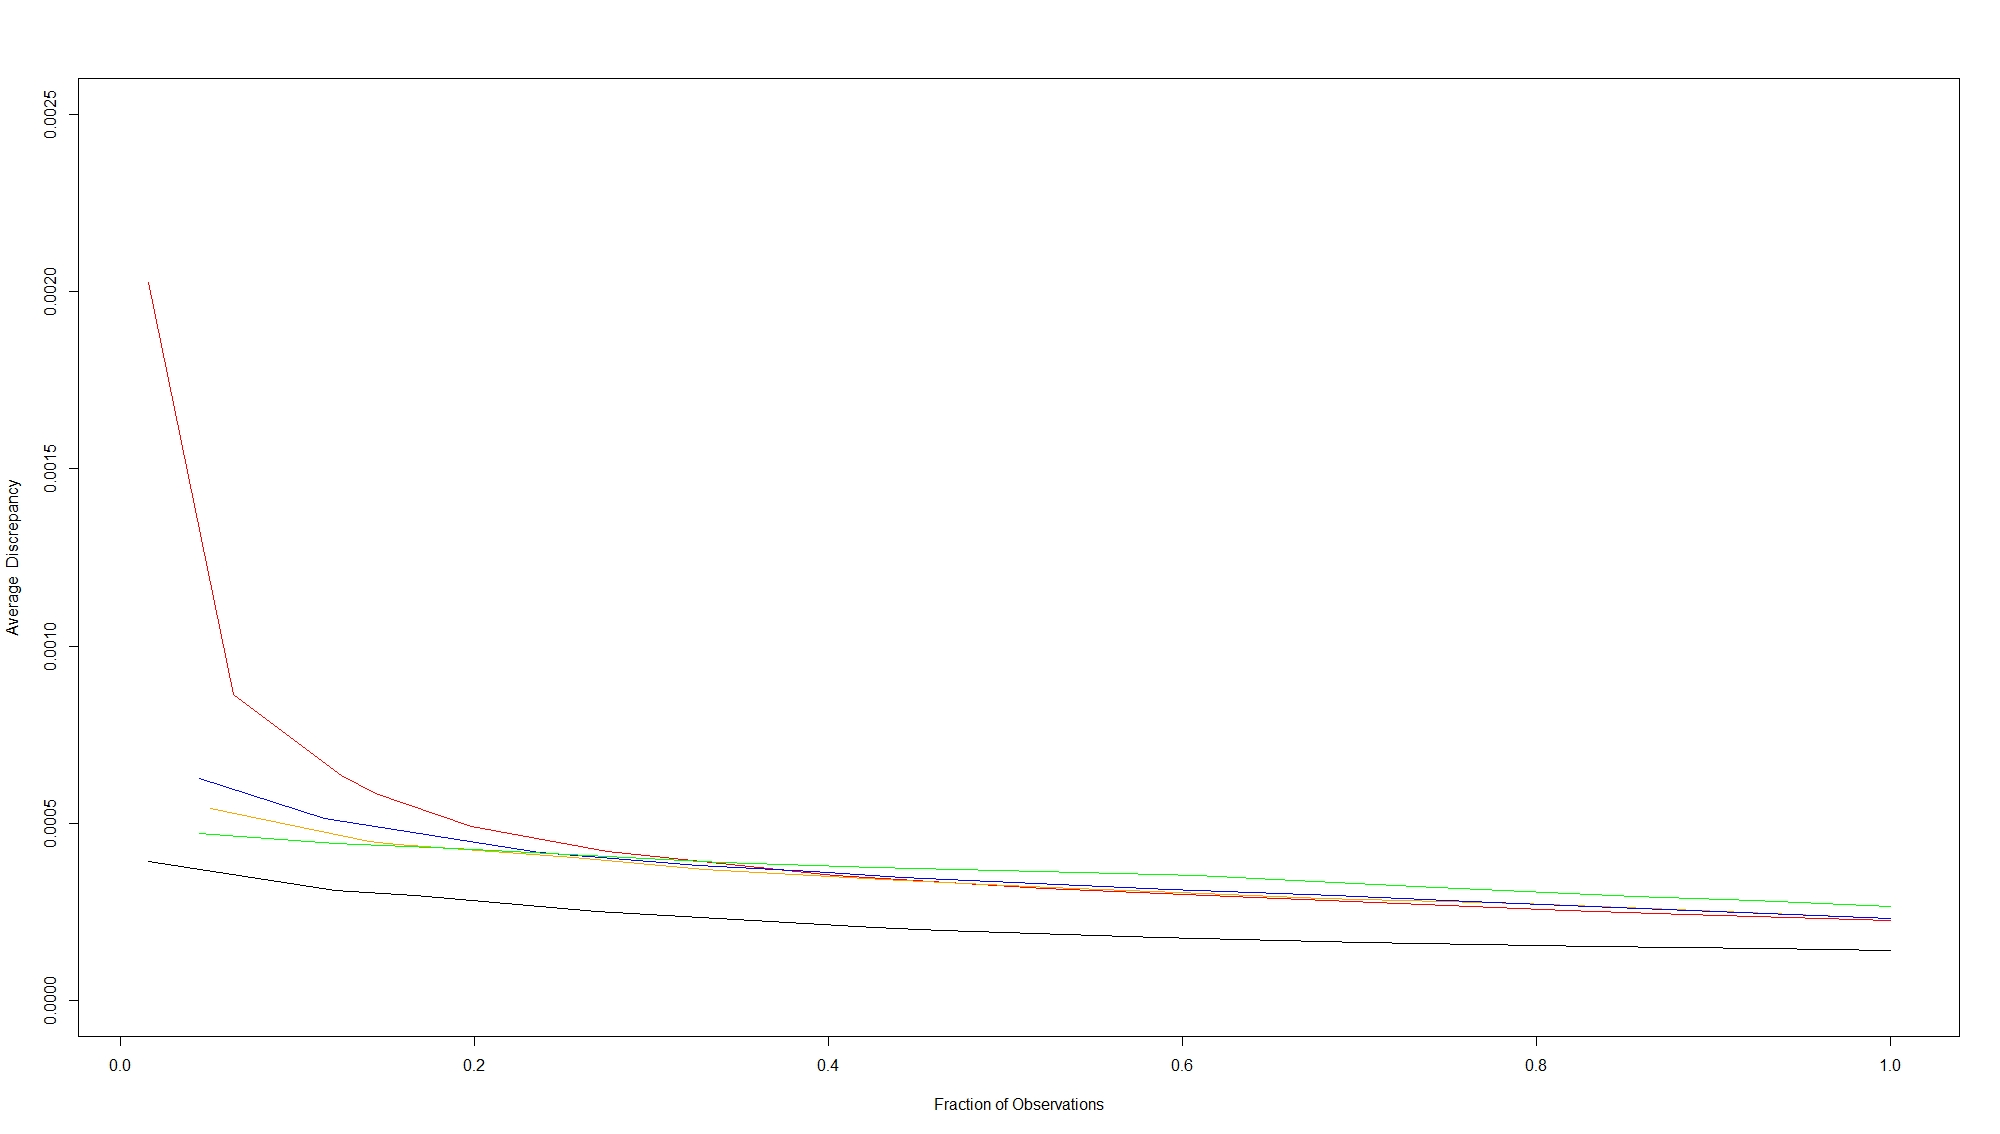
\includegraphics[width=0.31\textwidth]{lof_b}}\quad
\subfloat[Boosted model - Age 61-90]
{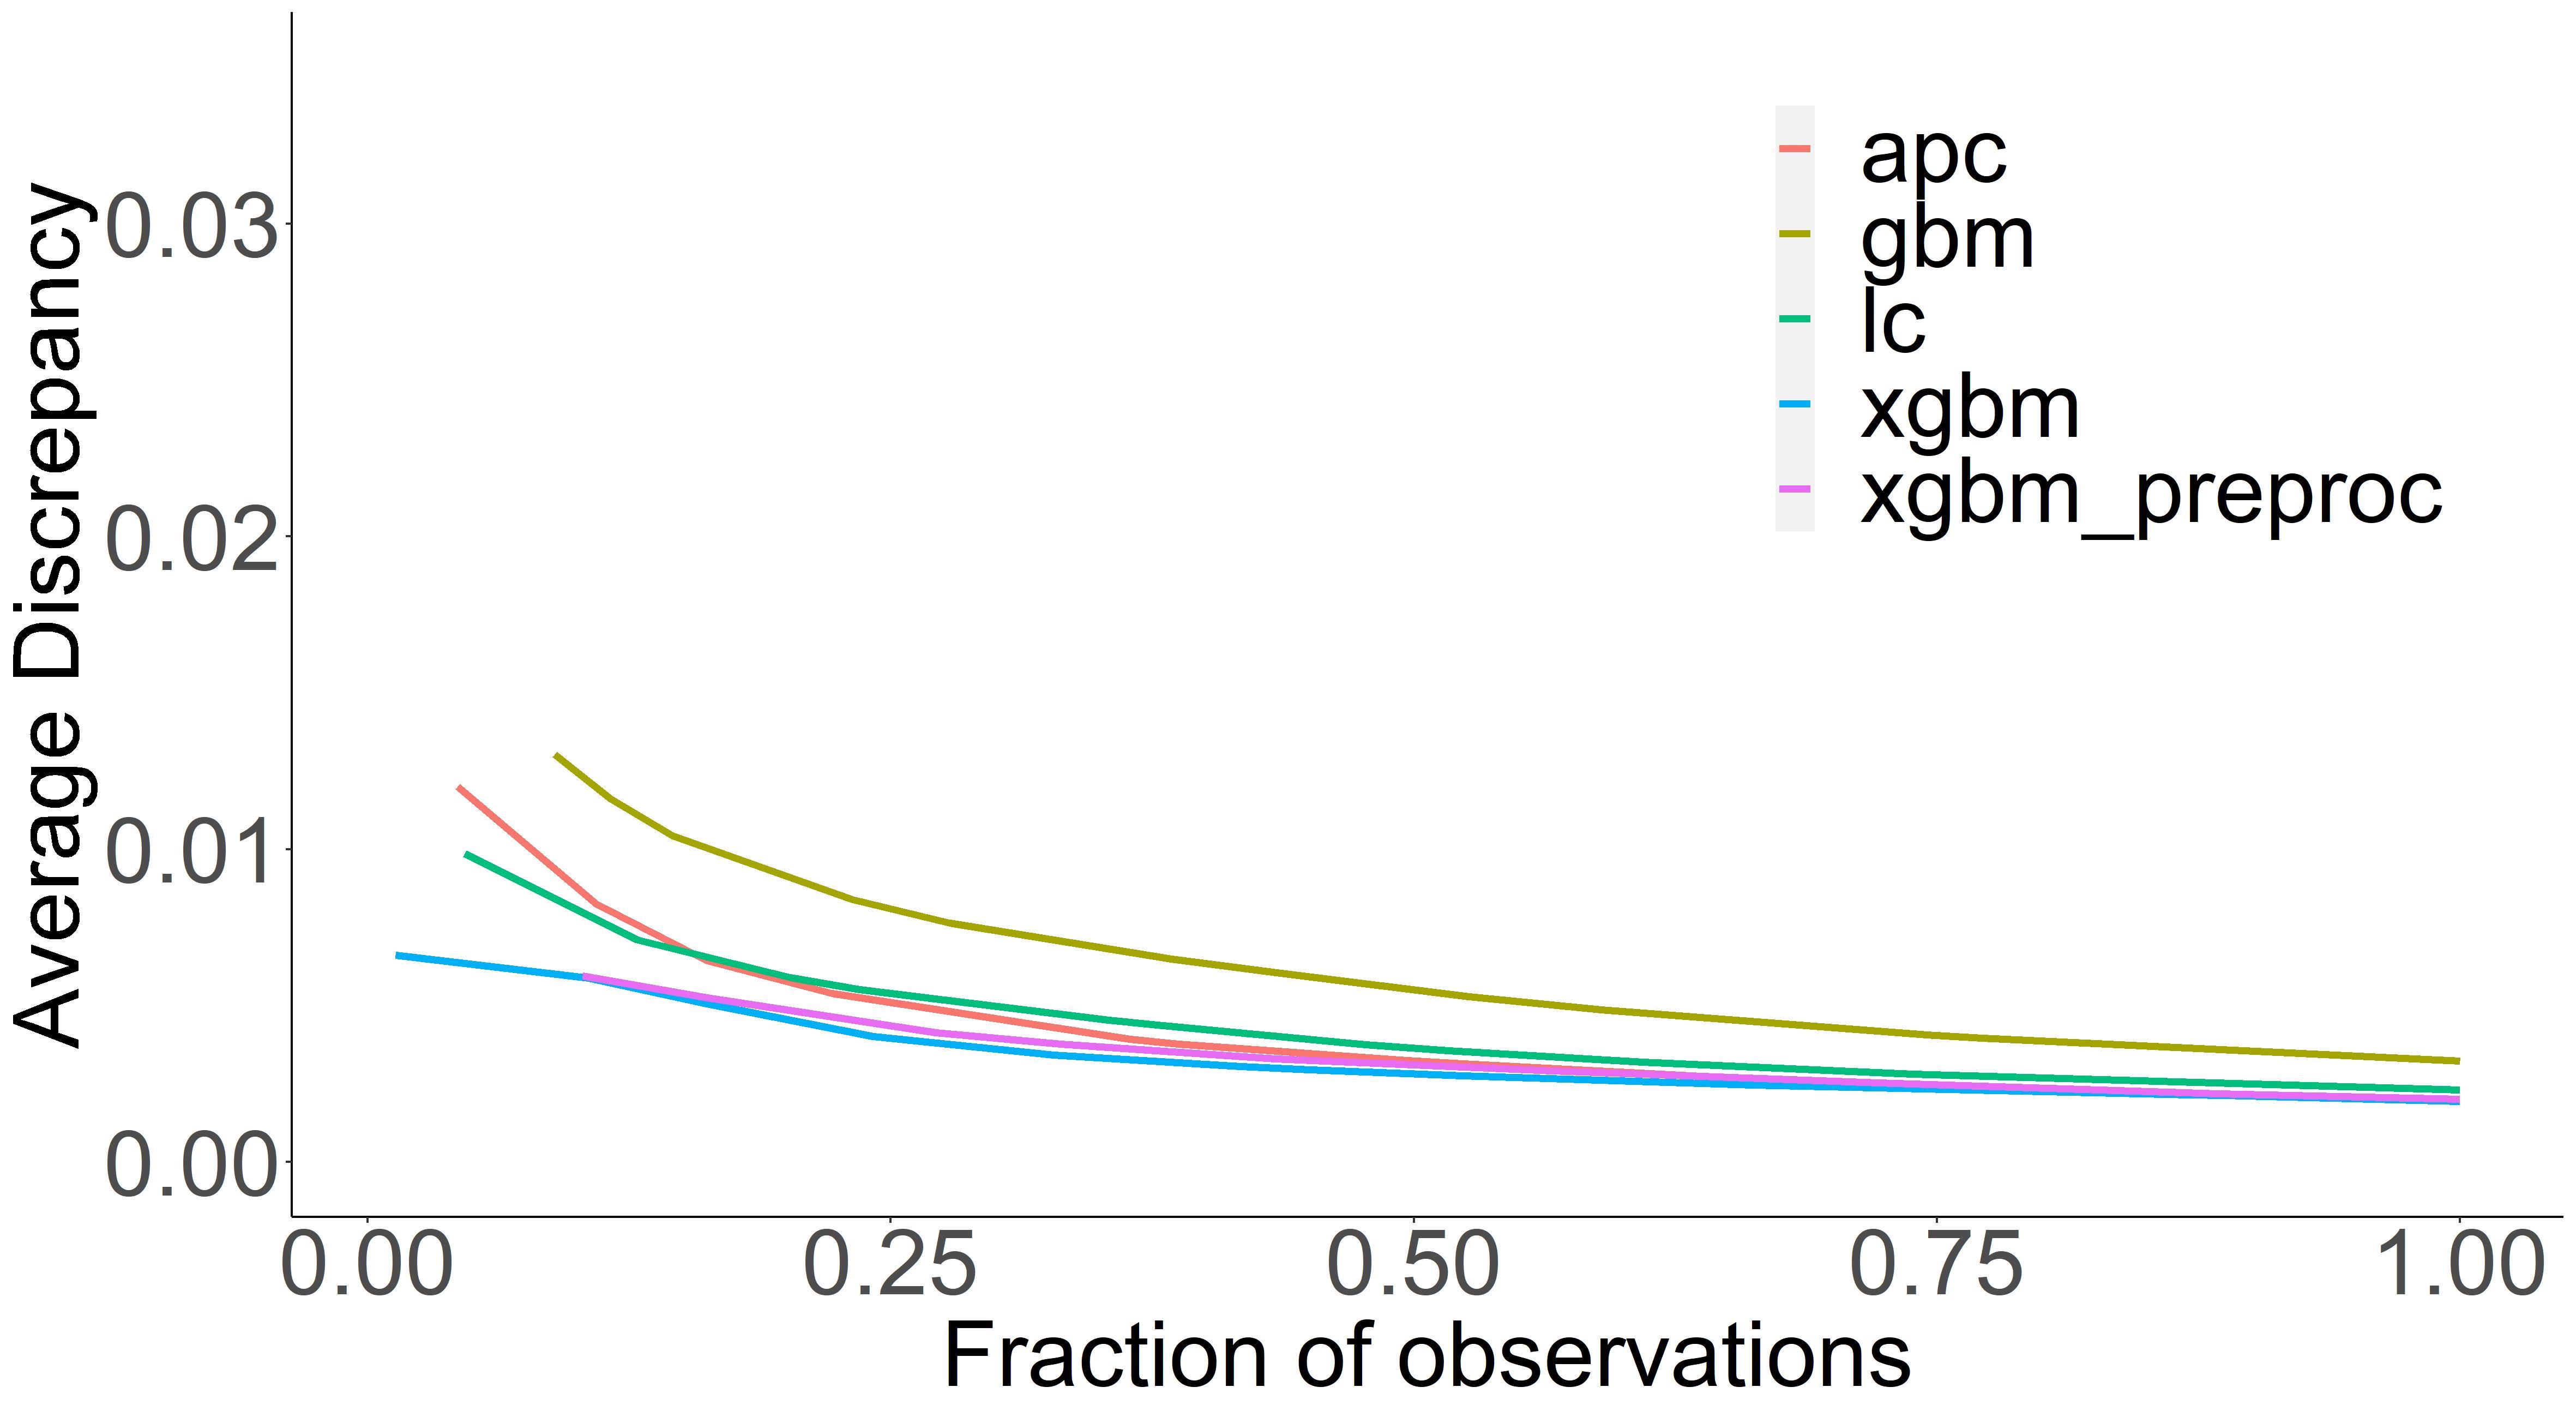
\includegraphics[width=0.31\textwidth]{lof_61_b}}
\caption{Lack-of-fit contrast curves for APC, LC, GBM, XGBM and XGBM prep.}
\label{fig:lof}
\end{figure}\\
%
Table \ref{tab:avecri} reports the values of the average discrepancy measure for both the base and the boosted models considered in the analysis. 
The APC and the XGBM base models provide the lowest average discrepancy values (0.000410 and 0.000417, respectively), which remain substantially unchanged after the Contrast boosting procedure.
The APC model shows the lowest value of $\bar{d}_m$ also for the age group 30-60, in line with the dynamics of the lack-of-fit curves depicted in panels (b) and (e) of Fig. \ref{fig:lof}.
However, the lack-of-fit curves provide more structured information than the average discrepancy, in particular, regarding how and how much $\bar{d}_m$ varies across the input space. For example, for the age group 61-90 in the base model (panel (c)), we can appreciate that the main difference among models (except for GBM, which is out of range) measured by the average discrepancy is caused by the high discrepancy regions (where the fraction of observation is less than about 0.20). 
For ages 61-90, the GBM base model shows the worst fitting to the observed mortality data. Although Contrast boosting produces a strong improvement in the discrepancy measure, GBM remains the worst model in terms of discrepancy. Contrast boosting is very effective also for the GBM model in the age group 30-60, as it heavily lowers (-30\%) the average discrepancy between observed and estimated values.
%
\begin{table}[ht]
\centering
\footnotesize
\begin{tabular}{|l|r|r|r|r|r|r|r|r|r|}
\hline
\multirow{2}{*}{Model} & \multicolumn{3}{c|}{Age 0-29} & \multicolumn{3}{c|}{Age 30-60} & \multicolumn{3}{c|}{Age 61-90} \\
\cline{2-10}
			&	Base 	&	Boosted 	& \% Change &	Base 	&	Boosted 	& \% Change &	Base 	&	Boosted	& \% Change\\
\hline
APC 	&	0.000410	&	0.000409	&	0\%	&	0.000145	&	0.000141	&	-3\%	&	0.002142	&	0.001948	&	-9\%	\\
LC 	&	0.000571	&	0.000568	&	0\%	&	0.000231	&	0.000232	&	0\%	&	0.002395	&	0.002314	&	-3\%	\\
GBM 	&	0.000473	&	0.000459	&	-3\%	&	0.000320	&	0.000225	&	-30\%	&	0.006525	&	0.003238	&	-50\%	\\
XGBM 	&	0.000417	&	0.000415	&	0\%	&	0.000240	&	0.000233	&	-3\%	&	0.001916	&	0.001940	&	1\%	\\
XGBM prep 	&	0.000500	&	0.000493	&	-1\%	&	0.000268	&	0.000265	&	-1\%	&	0.002003	&	0.002005	&	0\%	\\
\hline
\end{tabular}
\caption{Values of the average discrepancy $\bar{d}_m$ calculated on $m_{x,t}$ in the test set.}
\label{tab:avecri}
\end{table}\\
For a comparison with the average discrepancy, we also calculate the Root Mean Square Error (RMSE) and Mean Absolute Percentage Error (MAPE) on the base model and the boosted one. Intuitively, the three measures $\bar{d}_m$, RMSE, and MAPE quantify the "distance" between the estimates and the actual observations. 
However, the average discrepancy is an innovative measure summarizing the discrepancy over all the regions identified by the Contrast trees, while RMSE and MAPE are commonly used error measures calculated on the overall input space without distinguishing by region. 

By comparing Table \ref{tab:errors} showing the values of RMSE and MAPE with Table \ref{tab:avecri} reporting the values of the average discrepancy, we note a greater convergence of the error measures in the boosted models rather than in the base models. This result is intuitively straightforward since the boosted models are obtained by just reducing the discrepancy measure. 
%
\begin{table}[ht]
\centering
\footnotesize
\begin{tabular}{|l|l|r|r|r|r|r|r|r|r|r|}
\hline
\multirow{2}{*}{Error} & \multirow{2}{*}{Model} & \multicolumn{3}{c|}{Age 0-29} & \multicolumn{3}{c|}{Age 30-60} & \multicolumn{3}{c|}{Age 61-90} \\
\cline{3-11}
&			&	Base 	&	Boosted 	& \% Change &	Base 	&	Boosted 	& \% Change &	Base 	&	Boosted	& \% Change\\
\hline
\multirow{5}{*}{RMSE}  & APC 	&	0.002040	&	0.002039	&	0\%	&	0.000264	&	0.000263	&	0\%	&	0.004260	&	0.004139	&	-3\%	\\
& LC 	&	0.003471	&	0.003471	&	0\%	&	0.000491	&	0.000496	&	1\%	&	0.004258	&	0.004363	&	2\%	\\
& GBM 	&	0.001648	&	0.001647	&	0\%	&	0.000640	&	0.000455	&	-29\%	&	0.012248	&	0.005439	&	-56\%	\\
& XGBM 	&	0.001517	&	0.001515	&	0\%	&	0.000342	&	0.000338	&	-1\%	&	0.003260	&	0.003278	&	1\%	\\
& XGBM prep 	&	0.001939	&	0.001935	&	0\%	&	0.000391	&	0.000386	&	-1\%	&	0.003339	&	0.003345	&	0\%	\\
\hline
\multirow{2}{*}{Error} & \multirow{2}{*}{Model} & \multicolumn{3}{c|}{Age 0-29} & \multicolumn{3}{c|}{Age 30-60} & \multicolumn{3}{c|}{Age 61-90} \\
\cline{3-11}
&			&	Base 	&	Boosted 	& \% Change &	Base 	&	Boosted 	& \% Change &	Base 	&	Boosted	& \% Change\\
\hline
\multirow{5}{*}{MAPE}  & APC 			&	14.7\%	&	14.5\%	&	-1\%		&	4.5\%	&	4.3\%	&	-3\%		&	3.9\%	&	3.4\%	&	-14\% \\
& LC 			&	14.2\%	&	13.8\%	&	-3\%		&	7.2\%	&	7.1\%	&	-1\%		&	4.9\%	&	4.9\%	&	0\%	\\
& GBM 		&	23.4\%	&	18.8\%	&	-20\%	&	13.0\%	&	7.6\%	&	-41\%	&	18.3\%	&	9.2\%	&	-50\% \\
& XGBM 		&	15.9\%	&	15.3\%	&	-3\%		&	6.9\%	&	6.2\%	&	-10\%	&	3.7\%	&	3.8\%	&	2\%	\\
& XGBM prep 	&	20.0\%	&	18.2\%	&	-9\%		&	7.3\%	&	7.2\%	&	-1\%		&	3.6\%	&	3.6\%	&	0\%	\\
\hline
\end{tabular}
\caption{Values of the RMSE and MAPE calculated on $m_{x,t}$ in the test set.}
\label{tab:errors}
\end{table}\\
%
\color{blue}
We also calculate average discrepancy, RMSE, and MAPE on the logarithm of the central death rates (Tables \ref{tab:avecri_log}-\ref{tab:errors_log}). 
These measures assign a relatively large weight to errors at young ages, while error measures calculated on the central death rates assign a large weight to errors at older ages.
Indeed, for the age group 0-29, all the errors reported in Tables \ref{tab:avecri_log}-\ref{tab:errors_log} are significantly higher than those in Tables \ref{tab:avecri}-\ref{tab:errors}. 
The errors calculated on the logarithm of the central death rates highlight the ability of Contrast boosting to reduce the inaccuracy of GBM and XGBM-prep in fitting observed mortality at ages 0-29.\color{black} 
%
\begin{table}[ht]
\centering
\footnotesize
\begin{tabular}{|l|r|r|r|r|r|r|r|r|r|}
\hline
\multirow{2}{*}{Model} & \multicolumn{3}{c|}{Age 0-29} & \multicolumn{3}{c|}{Age 30-60} & \multicolumn{3}{c|}{Age 61-90} \\
\cline{2-10}
			&	Base 	&	Boosted 	& \% Change &	Base 	&	Boosted 	& \% Change &	Base 	&	Boosted	& \% Change\\
\hline
APC 			&	0.149906	&	0.148218	&	-1\%		&	0.040837	&	0.040276		&	-1\%		&	0.036633	&	0.035584	&	-3\%	\\
LC 			&	0.151968	&	0.149051	&	-2\%		&	0.066676	&	0.070489		&	6\%		&	0.042757	&	0.039114	&	-9\%	\\
GBM 		&	0.292233	&	0.260784	&	-11\%	&	0.109899	&	0.052510		&	-52\%	&	0.118491	&	0.052240	&	-56\% \\
XGBM 		&	0.195720	&	0.191478	&	-2\%		&	0.066986	&	0.062600		&	-7\%		&	0.036712	&	0.036779	&	0\%	\\
XGBM prep 	&	0.207129	&	0.186137	&	-10\%	&	0.072703	&	0.072571		&	0\%		&	0.035729	&	0.035505	&	-1\%	\\
\hline
\end{tabular}
\caption{Values of the average discrepancy $\bar{d}_m$ calculated on $\log{\left(m_{x,t}\right)}$ in the test set.}
\label{tab:avecri_log}
\end{table}\\
%
\begin{table}[ht]
\centering
\footnotesize
\begin{tabular}{|l|l|r|r|r|r|r|r|r|r|r|}
\hline
\multirow{2}{*}{Error} & \multirow{2}{*}{Model} & \multicolumn{3}{c|}{Age 0-29} & \multicolumn{3}{c|}{Age 30-60} & \multicolumn{3}{c|}{Age 61-90} \\
\cline{3-11}
&			&	Base 	&	Boosted 	& \% Change &	Base 	&	Boosted 	& \% Change &	Base 	&	Boosted	& \% Change\\
\hline
\multirow{5}{*}{RMSE}  & APC 		&	0.197670	&	0.197502	&	0\%		&	0.062659	&	0.062708	&	0\%	&	0.049847	&	0.049678	&	0\%	\\
& LC 		&	0.237064	&	0.232791	&	-2\%		&	0.101946	&	0.106096	&	4\%	&	0.060798	&	0.056322	&	-7\%	\\
& GBM 		&	0.707561	&	0.694538	&	-2\%		&	0.182743	&	0.071172	&	-61\%	&	0.233815	&	0.081485	&	-65\%	\\
& XGBM 		&	0.503457	&	0.496244	&	-1\%		&	0.089719	&	0.084808	&	-5\%	&	0.053659	&	0.053511	&	0\%	\\
& XGBM prep 	&	0.306517	&	0.272596	&	-11\%	&	0.096897	&	0.097073	&	0\%	&	0.048344	&	0.048111	&	0\%	\\
\hline
\multirow{2}{*}{Error} & \multirow{2}{*}{Model} & \multicolumn{3}{c|}{Age 0-29} & \multicolumn{3}{c|}{Age 30-60} & \multicolumn{3}{c|}{Age 61-90} \\
\cline{3-11}
&			&	Base 	&	Boosted 	& \% Change &	Base 	&	Boosted 	& \% Change &	Base 	&	Boosted	& \% Change\\
\hline
\multirow{5}{*}{MAPE}  & APC 	&	2.1\%	&	2.2\%	&	0\%		&	0.8\%	&	0.8\%	&	0\%		&	1.4\%	&	1.2\%	&	1\%	\\
& LC 		&	2.1\%	&	2.1\%	&	-2\%		&	1.2\%	&	1.3\%	&	5\%		&	1.6\%	&	1.6\%	&	1\%	\\
& GBM 		&	3.5\%	&	3.1\%	&	-12\%	&	1.9\%	&	0.9\%	&	-52\%	&	4.7\%	&	5.6\%	&	2\%	\\
& XGBM 		&	2.6\%	&	2.5\%	&	-1\%		&	1.2\%	&	1.1\%	&	-4\%		&	1.2\%	&	1.3\%	&	1\%	\\
& XGBM prep 	&	2.8\%	&	2.7\%	&	-3\%		&	1.2\%	&	1.2\%	&	0\%		&	1.2\%	&	1.2\%	&	1\%	\\\hline
\end{tabular}
\caption{Values of the RMSE and MAPE calculated on $\log{\left(m_{x,t}\right)}$ in the test set.}
\label{tab:errors_log}
\end{table}\\
%
\color{blue} 
The most interesting feature of the application of Contrast trees to the field of mortality estimate is the automatic identification of the regions of the predictors' space where a given model provides high discrepancy values for certain combinations of ages-years obtained by comparing the model estimates with the observed mortality rates.
These regions can be easily detected and possibly interpreted, providing a further explanation of the model performances as well as helping to assess whether a model can be reliable or not. Fig. \ref{fig:CT} and Fig. \ref{fig:CT2} show the heatmap of all the error regions for the base model and the boosted one, respectively. \color{black} Low discrepancy regions are painted in green, while high discrepancy regions are painted in red. 
For the sake of plot readability, we colored in purple the regions presenting a discrepancy value exceeding 3e-04, 6e-04, and 0.008 for the age groups 0-29, 30-60, and 61-90, respectively.

\color{blue} We can generally observe that the regions’ width and shape change from model to model. Some regions show remarkable mortality estimation errors in specific age groups, others in specific intervals of years, others in a specific range of cohorts. 
All the models considered show high discrepancy values in the first year of age (Fig. \ref{fig:CT}, age group 0-29, left panels), confirming the difficulty of adequately estimating the mortality of newborns. This situation remains unchanged after the application of Contrast boosting, which, in this case, seems to be not effective (Fig. \ref{fig:CT2}, age group 0-29, left panels).
For the age group 30-60 in the base model (Fig. \ref{fig:CT}, central panels), the two XGBM models show high discrepancy values after age 45-46, while GBM in the years 2000-2018. The LC model instead evidences high errors in estimating the mortality of cohorts born between 1920 and 1932. Considering the 61-90 age group (Fig. \ref{fig:CT}, right panels), we notice that the GBM model continues to fail in estimating mortality rates in the years 2000-2018, while the LC model (and also APC) mortality rates in the cohorts born between 1920 and 1932.
By comparing the results for the base models (Fig. \ref{fig:CT}) with those for the boosted ones (Fig. \ref{fig:CT2}), we observe a clear effect of boosting on the GBM model for the 30-60 and 61-90 age groups and the XGBM for the 30-60 age group. \color{black} 
\begin{figure}%[H]
\centering
\subfloat[APC (left: age 0-29; centre: age 30-60 right: age 61-90)]
{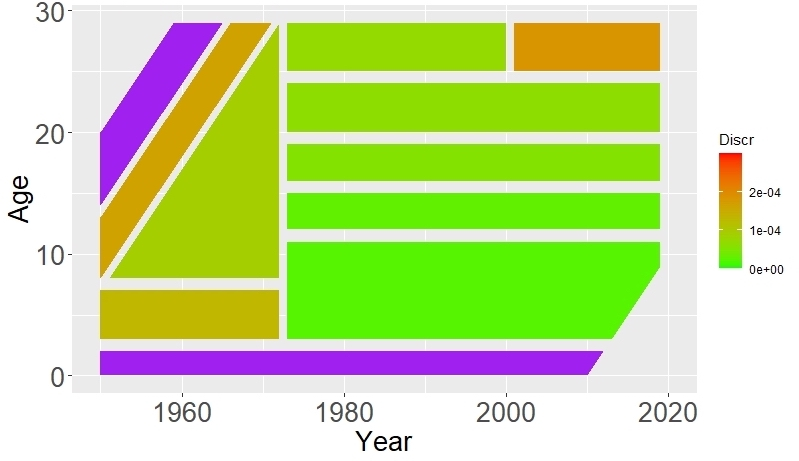
\includegraphics[width=0.32\textwidth]{apc_0.jpeg}
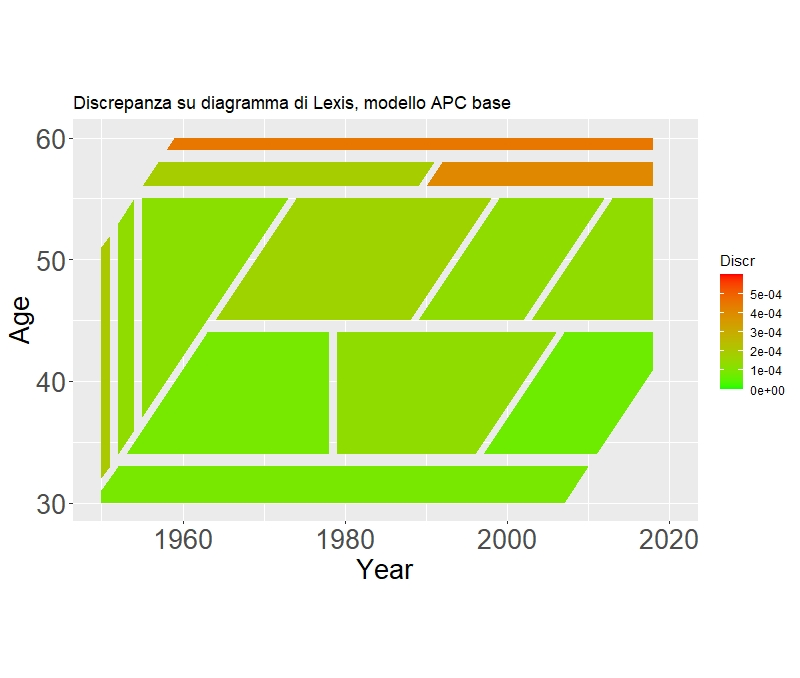
\includegraphics[width=0.32\textwidth]{apc.jpeg}
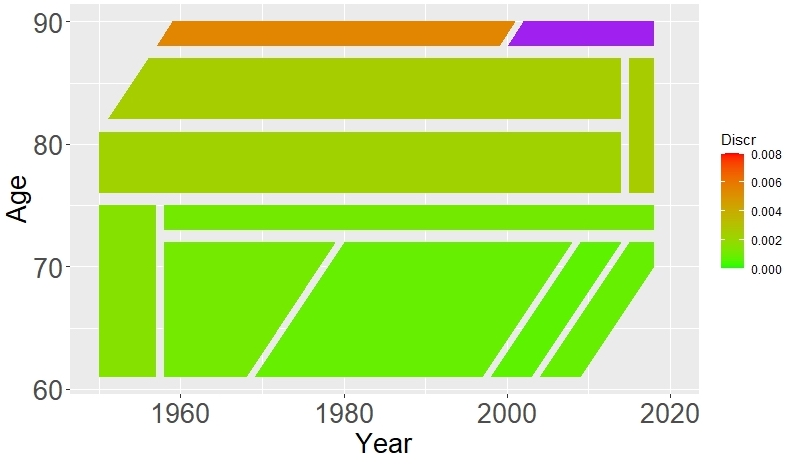
\includegraphics[width=0.32\textwidth]{apc_61.jpeg}}\\
\subfloat[LC (left: age 0-29; centre: age 30-60 right: age 61-90)]
{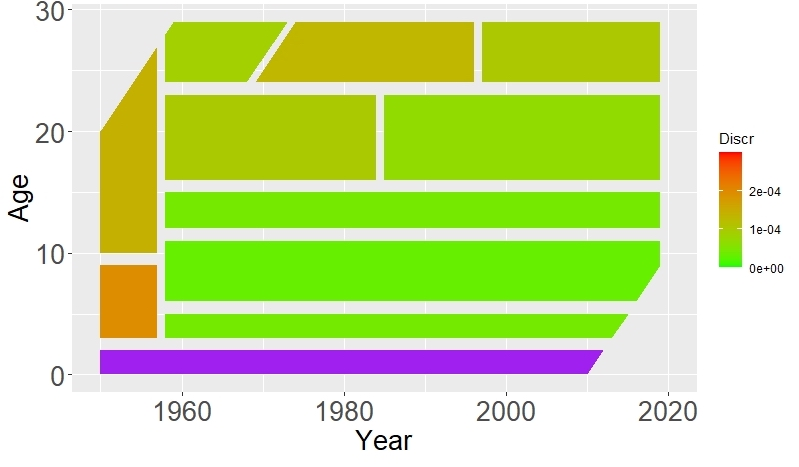
\includegraphics[width=0.32\textwidth]{lc_0.jpeg}
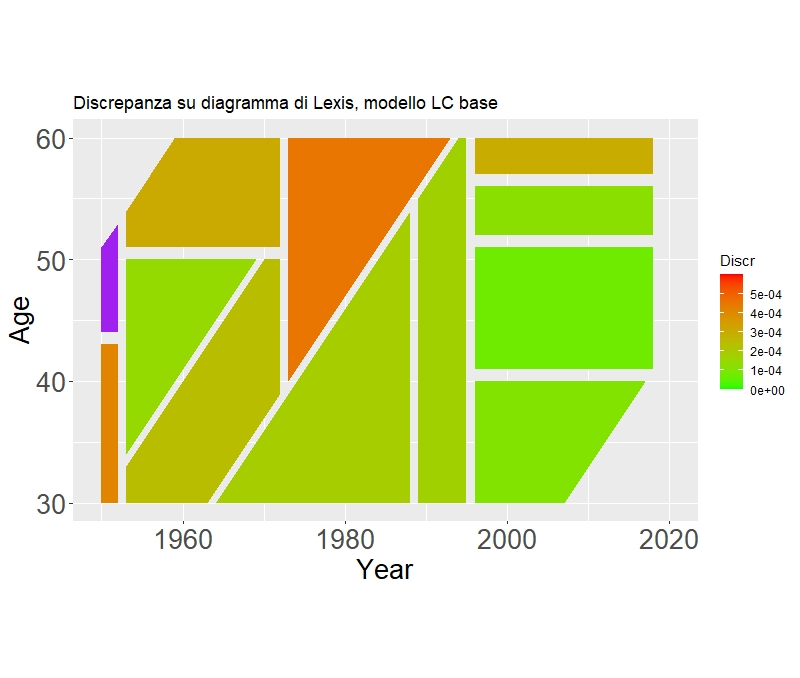
\includegraphics[width=0.32\textwidth]{lc.jpeg}
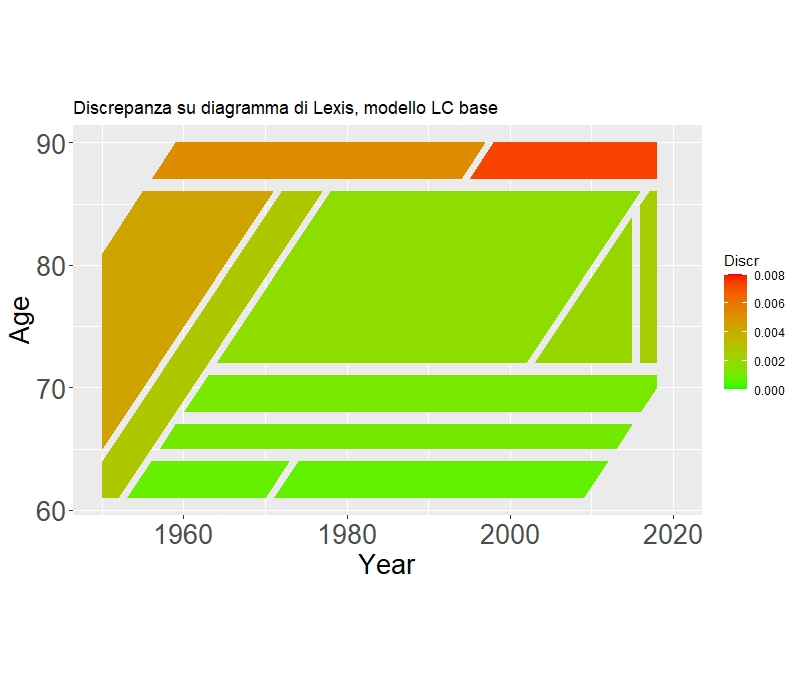
\includegraphics[width=0.32\textwidth]{lc_61.jpeg}}\\
\subfloat[GBM (left: age 0-29; centre: age 30-60 right: age 61-90)]
{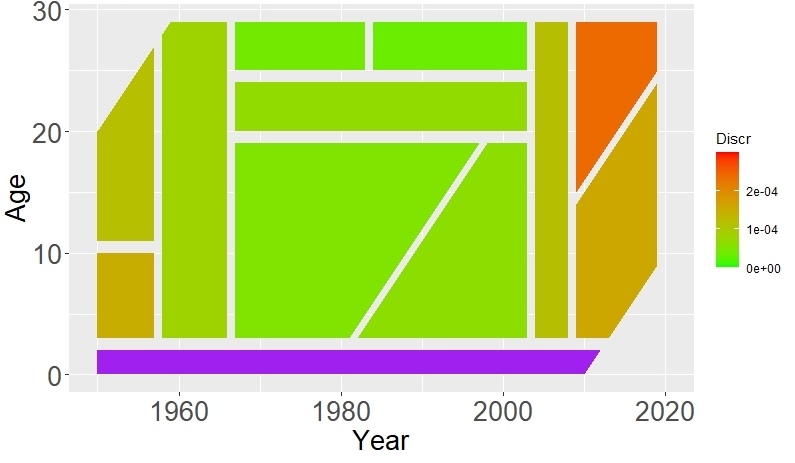
\includegraphics[width=0.32\textwidth]{gbm_0.jpeg}
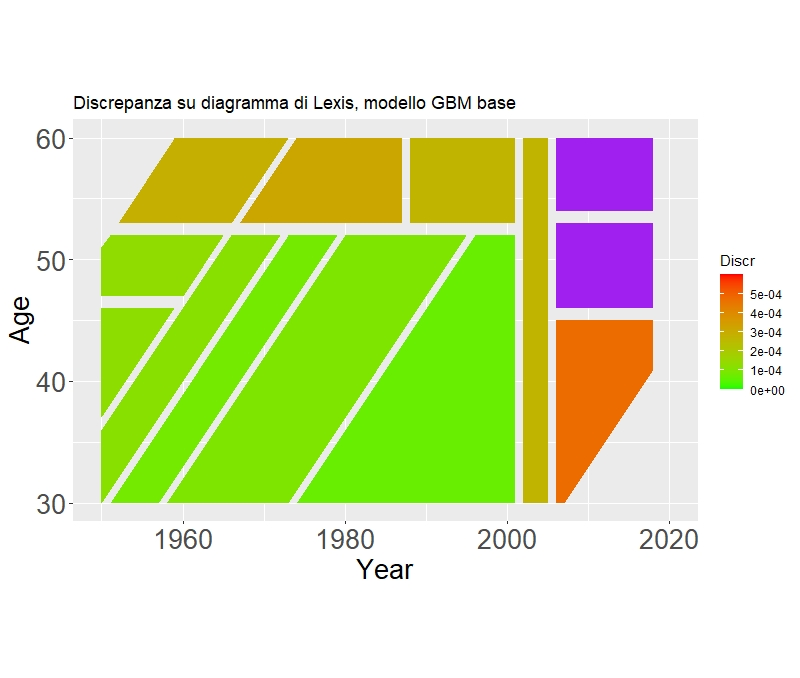
\includegraphics[width=0.32\textwidth]{gbm.jpeg}
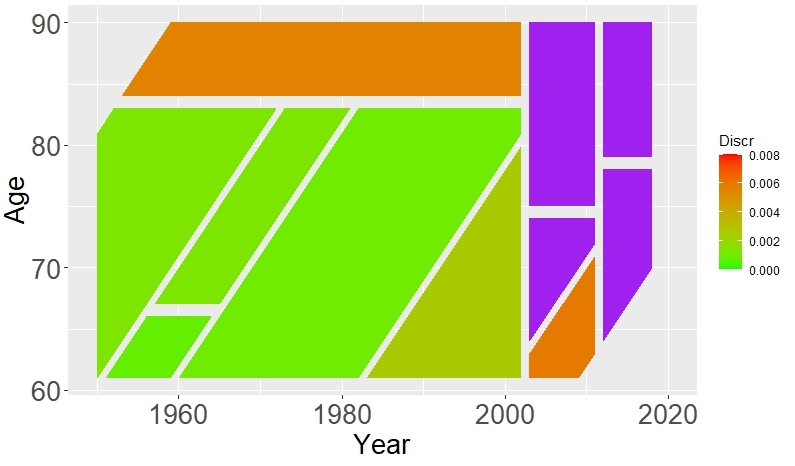
\includegraphics[width=0.32\textwidth]{gbm_61.jpeg}}\\
\subfloat[XGBM (left: age 0-29; centre: age 30-60 right: age 61-90)]
{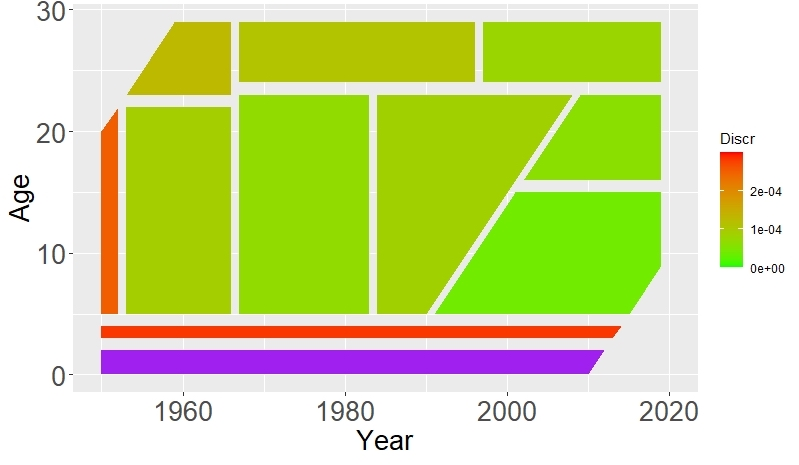
\includegraphics[width=0.32\textwidth]{xgbm_0.jpeg}
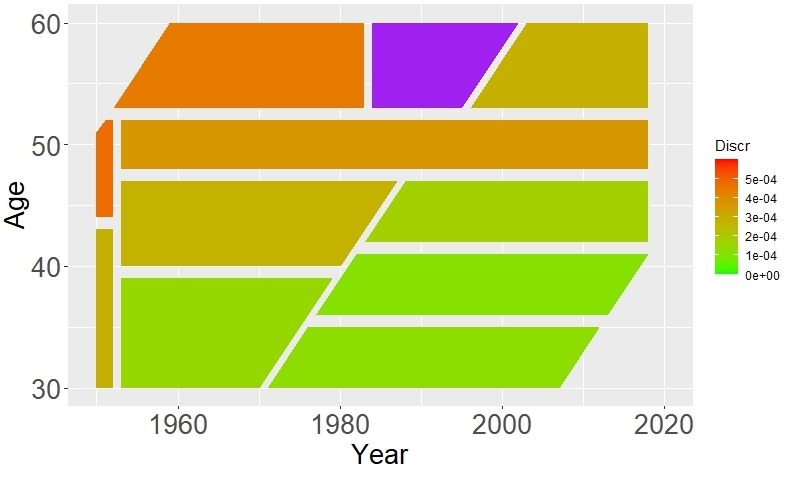
\includegraphics[width=0.32\textwidth]{xgbm.jpeg}
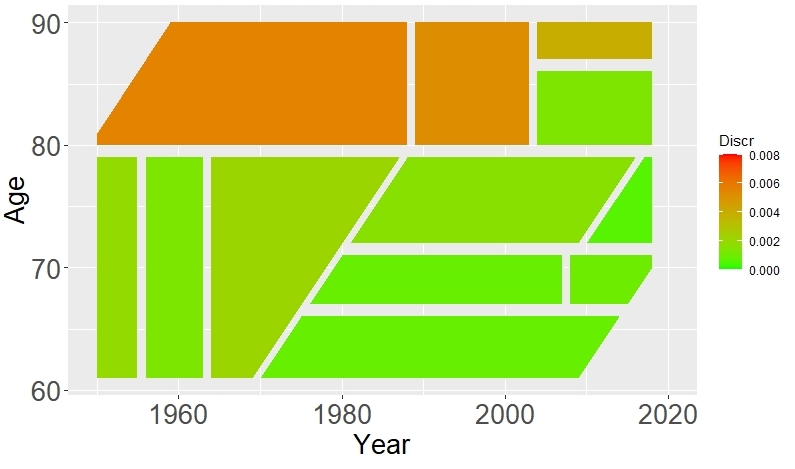
\includegraphics[width=0.32\textwidth]{xgbm_61.jpeg}}\\
\subfloat[XGM prep (left: age 0-29; centre: age 30-60 right: age 61-90)]
{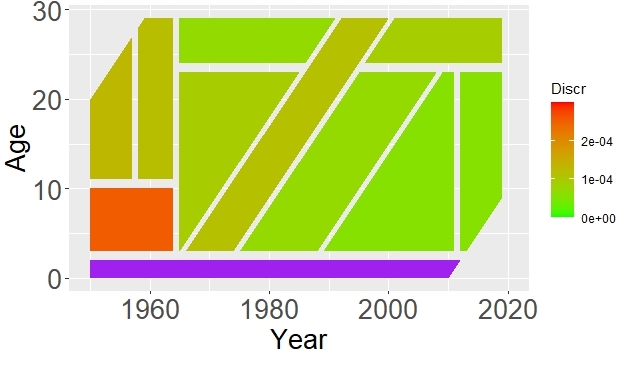
\includegraphics[width=0.32\textwidth]{xgbm_preproc_0.jpeg}
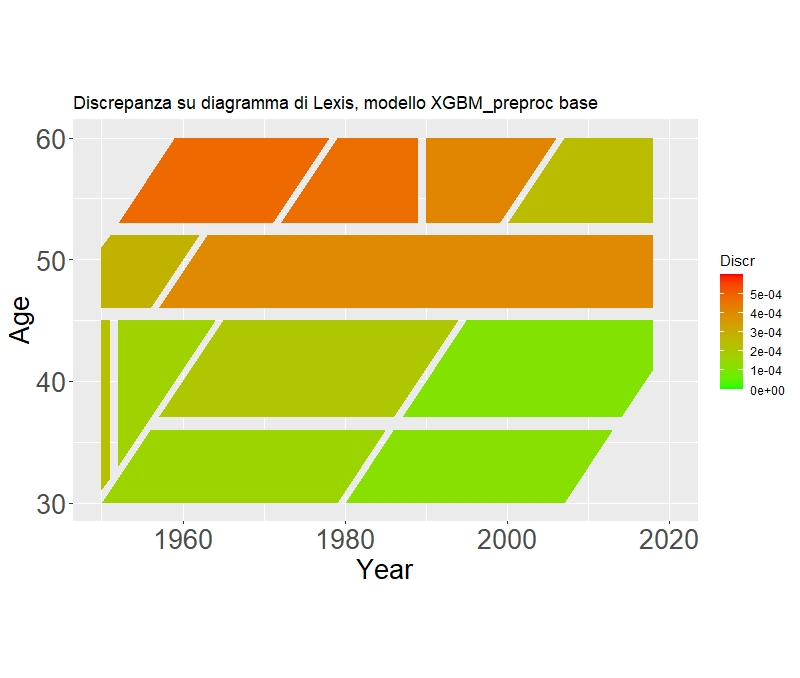
\includegraphics[width=0.32\textwidth]{xgbm_preproc.jpeg}
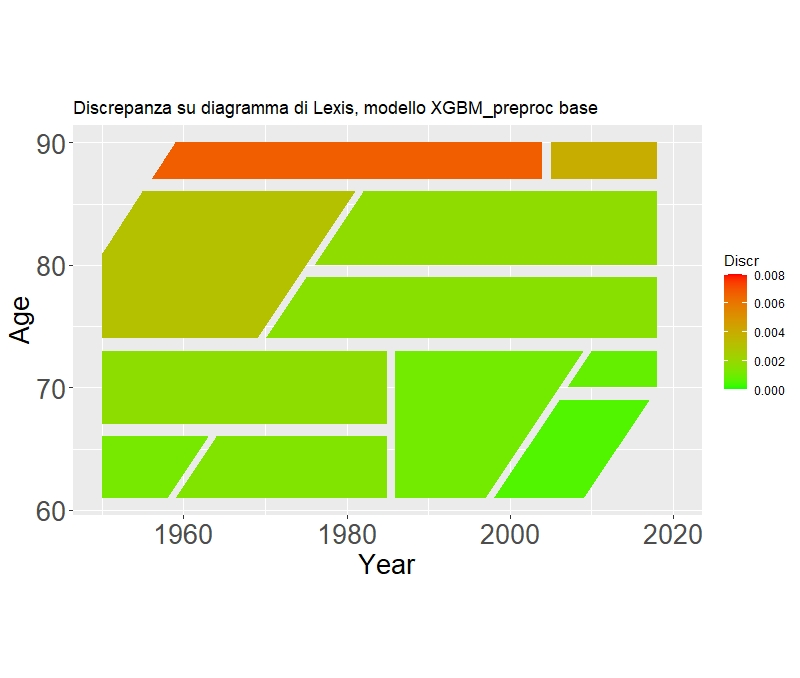
\includegraphics[width=0.32\textwidth]{xgbm_preproc_61.jpeg}}
\caption{Contrast trees regions, Base model. Years 1950-2018. Regions presenting a discrepancy value exceeding 3e-04 (age 0-29), 6e-04 (age 30-60), and 0.008 (61-90) are colored in purple.}
\label{fig:CT}
\end{figure}
%
\begin{figure}%[H]
\centering
\subfloat[APC (left: age 0-29; centre: age 30-60 right: age 61-90)]
{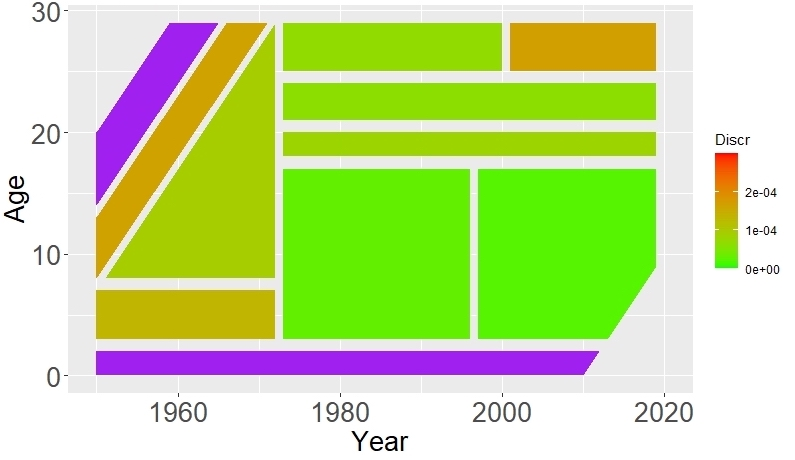
\includegraphics[width=0.32\textwidth]{apc_0_b.jpeg}
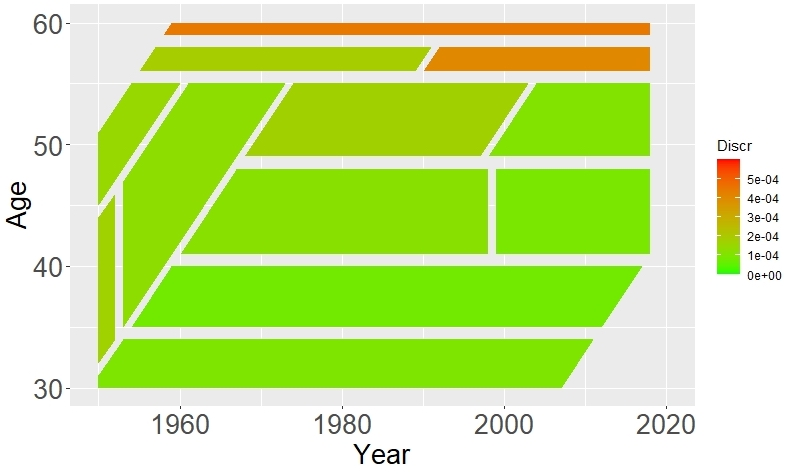
\includegraphics[width=0.32\textwidth]{apc_b.jpeg}
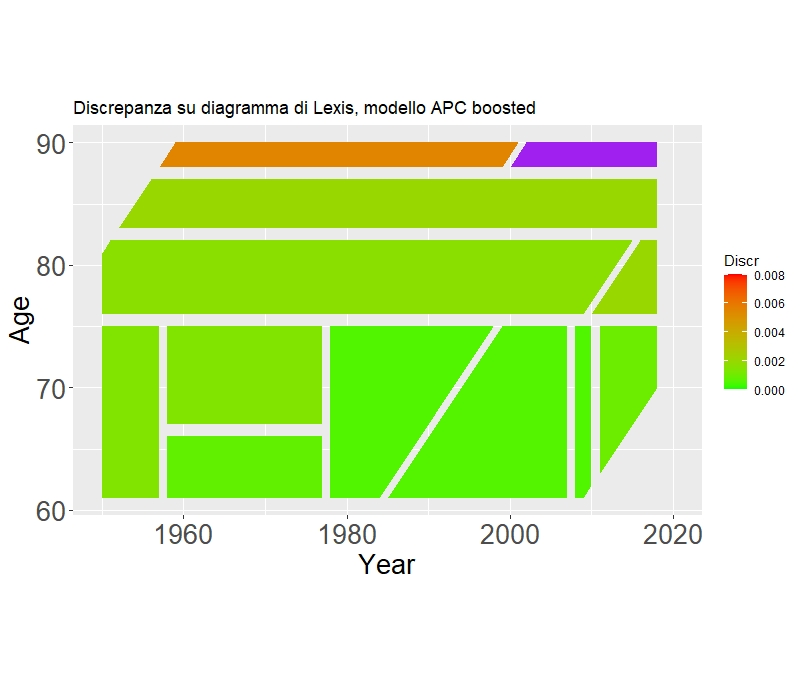
\includegraphics[width=0.32\textwidth]{apc_61_b.jpeg}}\\
\subfloat[LC (left: age 0-29; centre: age 30-60 right: age 61-90)]
{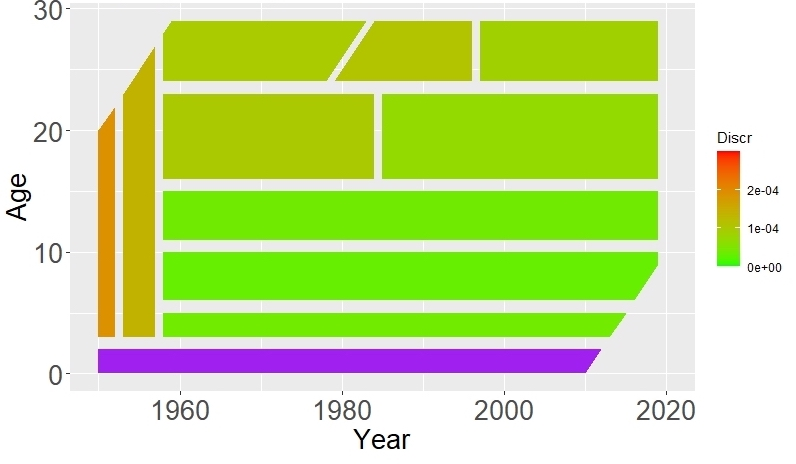
\includegraphics[width=0.32\textwidth]{lc_0_b.jpeg}
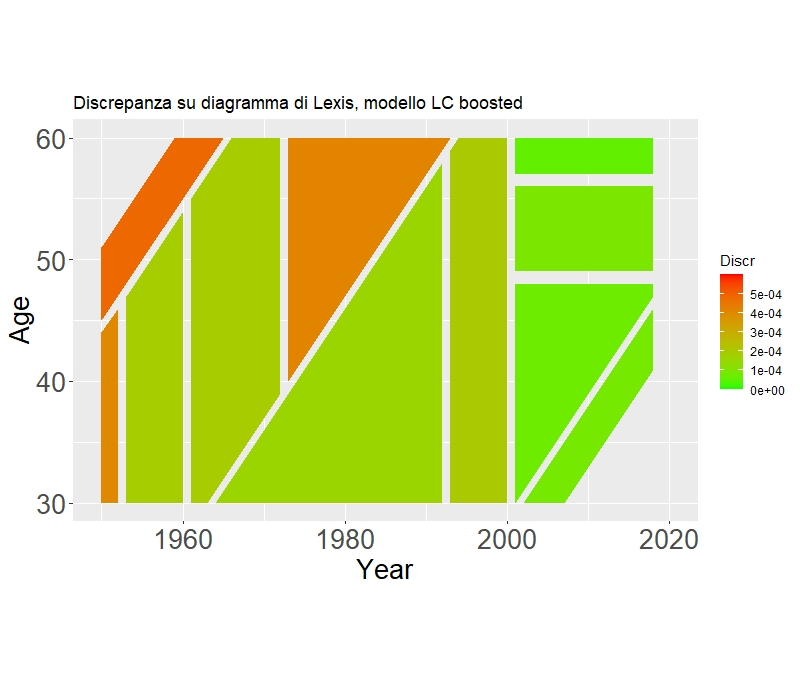
\includegraphics[width=0.32\textwidth]{lc_b.jpeg}
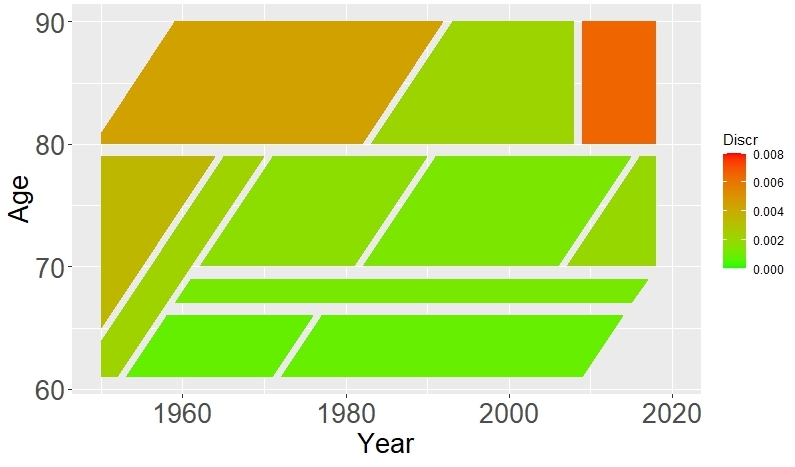
\includegraphics[width=0.32\textwidth]{lc_61_b.jpeg}}\\
\subfloat[GBM (left: age 0-29; centre: age 30-60 right: age 61-90)]
{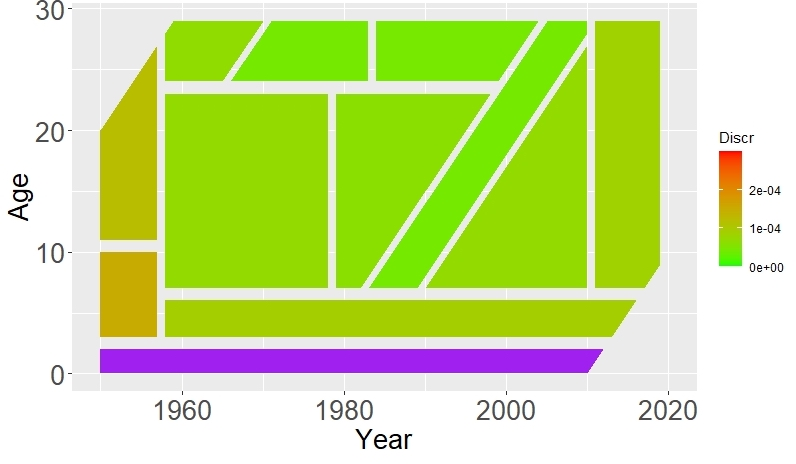
\includegraphics[width=0.32\textwidth]{gbm_0_b.jpeg}
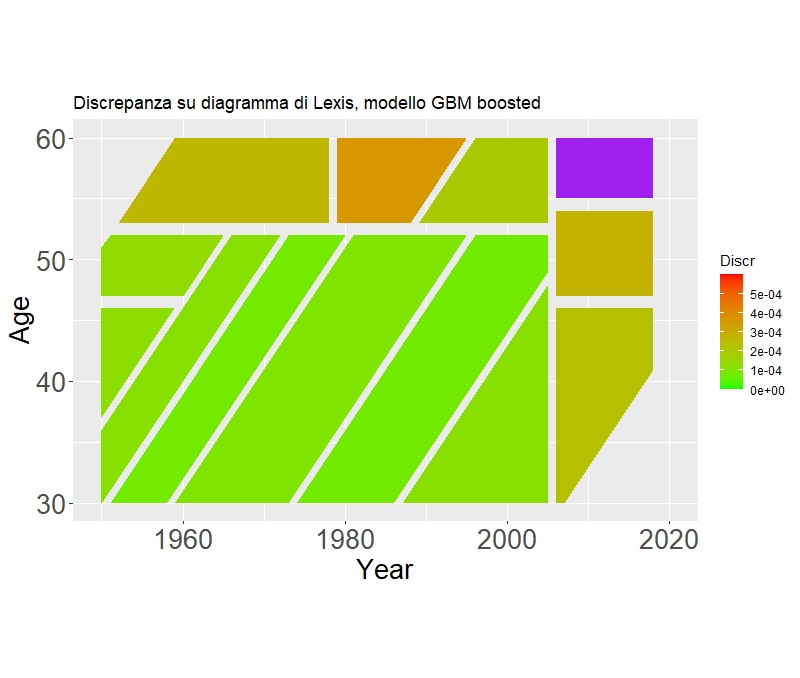
\includegraphics[width=0.32\textwidth]{gbm_b.jpeg}
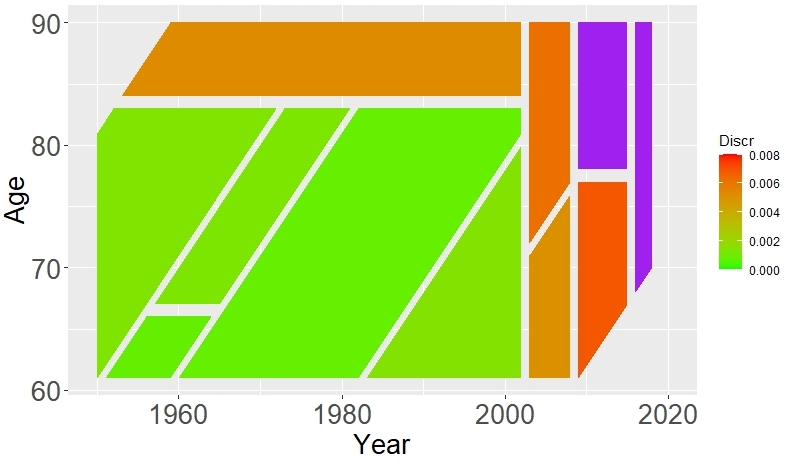
\includegraphics[width=0.32\textwidth]{gbm_61_b.jpeg}}\\
\subfloat[XGBM (left: age 0-29; centre: age 30-60 right: age 61-90)]
{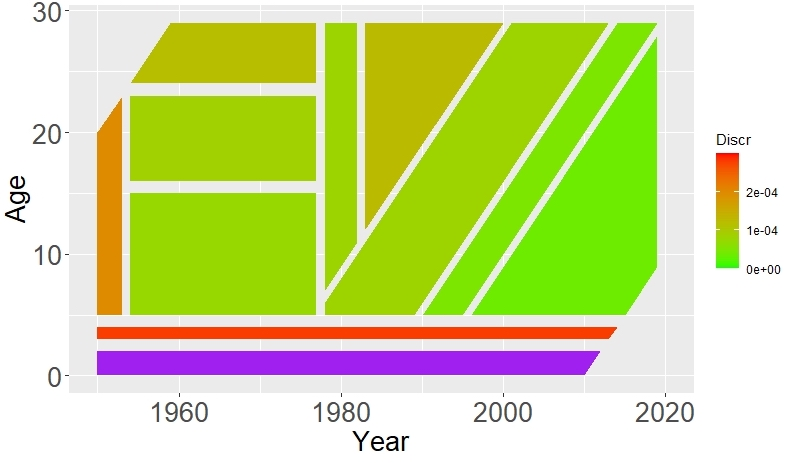
\includegraphics[width=0.32\textwidth]{xgbm_0_b.jpeg}
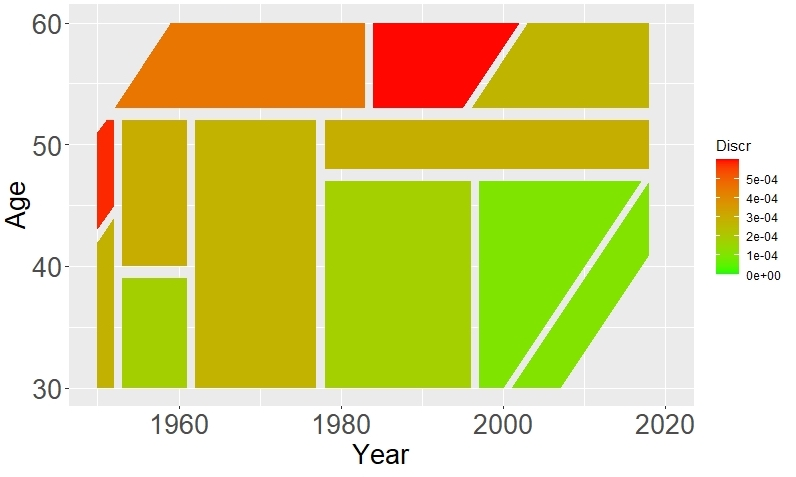
\includegraphics[width=0.32\textwidth]{xgbm_b.jpeg}
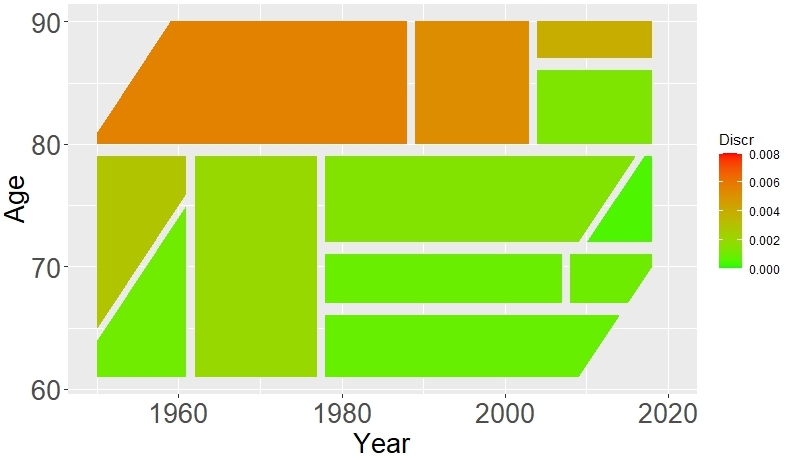
\includegraphics[width=0.32\textwidth]{xgbm_61_b.jpeg}}\\
\subfloat[XGM prep (left: age 0-29; centre: age 30-60 right: age 61-90)]
{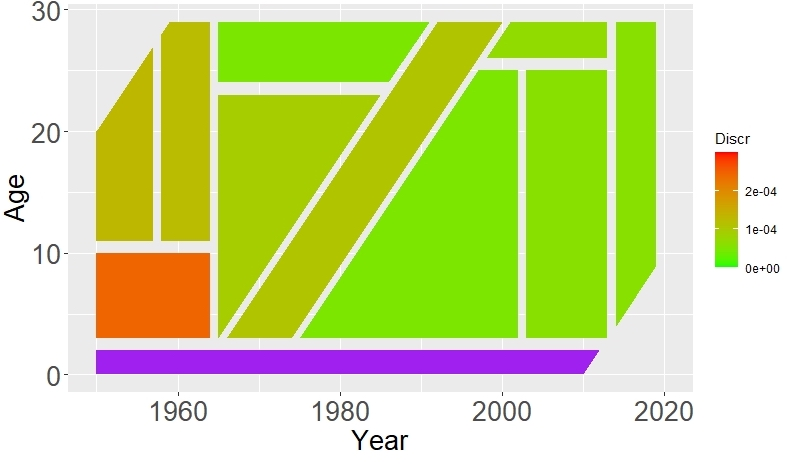
\includegraphics[width=0.32\textwidth]{xgbm_preproc_0_b.jpeg}
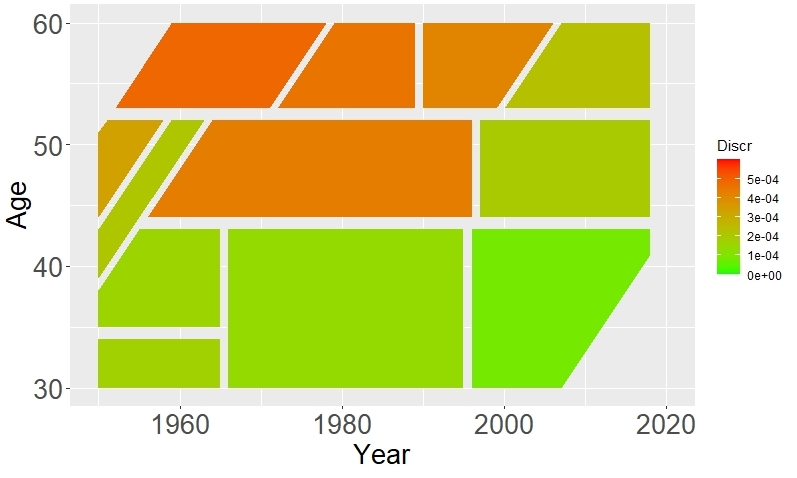
\includegraphics[width=0.32\textwidth]{xgbm_preproc_b.jpeg}
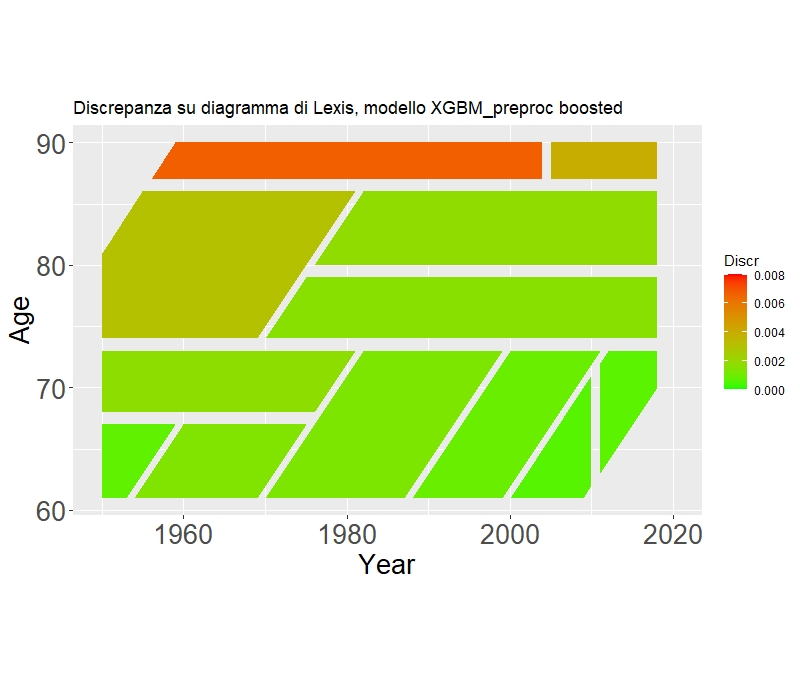
\includegraphics[width=0.32\textwidth]{xgbm_preproc_61_b.jpeg}}
\caption{Contrast trees regions, Boosted model. Years 1950-2018. Regions presenting a discrepancy value exceeding 3e-04 (age 0-29), 6e-04 (age 30-60), and 0.008 (61-90) are colored in purple.}
\label{fig:CT2}
\end{figure}
%\subsubsection*{Third-level section}
 %Topical subheadings are allowed.

%-------------------------------------------------------------
\section*{Discussion}
%-------------------------------------------------------------
%\textit{The Discussion should be succinct and must not contain subheadings.}\\
\textcolor{blue}{Evaluating, and thus eventually improving, the fit of mortality models is crucial for both demographers and actuaries. 
Indeed, in particular situations, common in actuarial practice, data quality can turn the mortality estimate difficult. 
A prime example is the case of small subpopulations where a common method such as the Lee-Carter may not guarantee reliable estimation. In this sense, our proposal fills the gap between mortality modeling and model diagnostics, particularly for nontraditional modeling as a machine learning framework.\\
Contrast trees consist of a general method based on machine learning that can be applied to any model, expressed as a regression model, to evaluate the goodness of fit and identify the worst-performing regions in the input space. The main characteristic that discriminates this method from traditional diagnostic tools is automatically identifying the regions in which a given model produces a high error for certain combinations of ages and calendar years.
Well-known diagnostic tools often used in the literature to assess the goodness-of-fit of a mortality model, such as BIC and AIC, require the likelihood function, which is not available for machine learning models. Therefore, Contrast trees provide a unified approach for assessing and comparing the accuracy of traditional mortality models with machine learning algorithms.}\\
In Contrast trees, the detection of the regions in which a model worst performs can be considered an evolution of the standard analysis on residuals, in which the detection of the highest residuals is typically assigned to graphical analyzes using heatmaps and scatter plots \cite{CBD09,Villegas2018}, and to summary measures like RMSE and MAPE calculated on the overall input space and not by region.
Conversely, the decision tree structure of Contrast trees enables quantifying the discrepancy between the estimates provided by a model and the actual observations in each region identified by Contrast trees.

%-------------------------------------------------------------
%\bibliography{myref}
%-------------------------------------------------------------
\begin{thebibliography}{99}

\bibitem%[Alai and Sherris(2014)]
{Alai2014}
Alai, D.H., Sherris, M. (2014). Rethinking age-period-cohort mortality trend models. Scandinavian Actuarial Journal, 3: 208-227.

\bibitem%[Bongaarts(2005)]
{Bongaarts2005}
Bongaarts, J. (2005). Long-Range Trends in Adult Mortality: Models and Projection Methods. Demography, 42(1): 23-49.

\bibitem%[Booth and Tickle(2008)]
{Booth}
Booth, H., Tickle, L. (2008). Mortality modelling and forecasting: A review of methods. Annals of Actuarial Science, 3(1-2): 3-43. DOI: 10.1017/S1748499500000440.

\bibitem%[Brouhns et al.(2002)]
{BDV2002}
Brouhns, N., Denuit, M., Vermunt, J. (2002). A Poisson log-bilinear approach to the construction of projected life tables, Insurance: Mathematics and Economics, 31: 373-393.

\bibitem%[Chen et al.(2015)]
{Chen} 
Chen, T., He, T., Benesty, M., Khotilovich, V., Tang, Y., Cho, H. (2015). Xgboost: extreme gradient boosting. R package version 0.4-2, 1(4), 1-4.

\bibitem%[Cairns et al.(2006)]
{CBD06} 
Cairns, A.J.G., Blake, D., Dowd, K. (2006). A Two-Factor Model for Stochastic Mortality with Parameter Uncertainty: Theory and Calibration. Journal of Risk and Insurance, 73: 687-718.

\bibitem%[Cairns et al.(2008)]
{CBD08} 
Cairns, A.J.G., Blake, D., Dowd, K. (2008). Modelling and management of mortality risk: a review. Scandinavian Actuarial Journal, 73 (2-3): 79-113.

\bibitem%[Cairns et al.(2009)]
{CBD09} 
Cairns, A.J.G., Blake, D., Dowd, K., Coughlan, G.D., Epstein, D., Ong, A., Balevich, I. (2009). A quantitative comparison of stochastic mortality models using data from England and Wales and the United States. North American Actuarial Journal, 13: 1-35.

\bibitem%[Cairns et al.(2010)]
{Cairns2010}
Cairns, A.J.G., Blake, D., Dowd, K., Coughlan, G.D., Epstein, D., Khalaf-Allah, M. (2010). Evaluating the goodness of fit of stochastic mortality models. Insurance: Mathematics and Economics, 47(3): 255-265.

\bibitem%[Deprez et al.(2017)]
{Deprez} 
Deprez, P., Shevchenko, P.V., W\'uthrich, M.V (2017). Machine learning techniques for mortality modeling. European Actuarial Journal, 7: 337-352. https://doi.org/10.1007/s13385-017-0152-4.

\bibitem%[Djeundje et al.(2022)]
{Djeundje2022} 
Djeundje, V.B., Haberman, S., Bajekal, M. et al. (2022). The slowdown in mortality improvement rates 2011-2017: a multi-country analysis. European Actuarial Journal. DOI: 10.1007/s13385-022-00318-0

\bibitem%[Friedman(2001)]
{Friedman} 
Friedman, J.H. (2001). Greedy function approximation: A Gradient Boosting Machine. Annals of Statistics 29: 1189-1232.

\bibitem%[Friedman(2020)]
{Friedman2020}
Friedman, J.H. (2020). Contrast trees and distribution boosting. Proceedings of the National Academy of Sciences, 117 (35): 21175-21184. DOI: 10.1073/pnas.1921562117

\bibitem%[Friedman and Narasimhan(2020)]
{FriedmanNarasimhan2020}
Friedman, J.H., Narasimhan, B. (2020). conTree: Contrast Trees and Distribution Boosting. R package version 0.2-8.

\bibitem%[Lee and Carter(1992)]
{LC92}
Lee, R.D., Carter, L.R. (1992). Modeling and forecasting US mortality. Journal of the American statistical association, 87 (419): 659-671.

\bibitem%[Levantesi and Nigri(2020)]
{LevNi}
Levantesi, S., Nigri, A. (2020). A random forest algorithm to improve the Lee-Carter mortality forecasting: impact on q-forward. Soft Computing, 24: 8553-8567. DOI: 10.1007/s00500-019-04427-z

\bibitem%[Levantesi and Pizzorusso(2019)]
{LevPiz}
Levantesi S., Pizzorusso, V. (2019). Application of Machine Learning to Mortality Modeling and Forecasting. Risks, 7(1), 26. ISSN: 2227-9091. DOI:10.3390/risk7010026

\bibitem%[Li et al.(2009)]
{Li2009}
Li, J. S.H.,  Hardy, M. R., Tan, K. S. (2009). Uncertainty in mortality forecasting: an extension to the classical Lee-Carter approach. Astin Bulletin 39(1), 137-164.

\bibitem%[Pollard(1987)]
{Pollard}
Pollard, J.H. (1987). Projection of age-specific mortality rates. In: Population Bulletin of the United Nations 21/22: 55-69.

\bibitem%[Renshaw and Haberman(2006)]
{RH}
Renshaw, A.E. , Haberman, S. (2006). A cohort-based extension to the Lee-Carter model for mortality reduction factors. Insurance: Mathematics and Economics, 38 (3): 556–570.

\bibitem%[Richman and W\"uthrich(2021)]
{RichmanWuthrich}
Richman, R. and W\"uthrich, M. (2021). A neural network extension of the Lee-Carter model to multiple populations. Annals of Actuarial Science, 15: 346-366.

\bibitem%[Torri(2011)]
{Torri2011}
Torri, T. (2011). Building blocks for a mortality index: an international context. Eur. Actuar. J. 1 (Suppl 1): S127-S141

\bibitem%[Villegas et al.(2018)]
{Villegas2018}
Villegas, A.M., Kaishev, V. and Millossovich, P. (2018). StMoMo: An R Package for Stochastic Mortality Modelling. Journal of Statistical Software, 84 (3): 1-38.

\bibitem%[Willett(1999)]
{Willett1999}
Willett, P. (1999). Dissimilarity-based algorithms for selecting structurally diverse sets of compounds. Journal of Computational Biology, 6 (3-4): 447-457.
 
\end{thebibliography}


\section*{Author contributions}
Authors equally contributed to this work.

\section*{Data availability}
The dataset analyzed during the current study, referred to Human Mortality Database (HMD), is available at \url{https://www.mortality.org/}

\section*{Competing interests}
The authors declare no competing interests.

%-------------------------------------------------------------
\section*{Acknowledgements}
%-------------------------------------------------------------
%%%%%%%%%%%%%%%%%%%%%%%%%%%%%%
%\textit{Acknowledgements should be brief, and should not include thanks to anonymous referees and editors, or effusive comments. Grant or contribution numbers may be acknowledged.}
%%%%%%%%%%%%%%%%%%%%%%%%%%%%%%
A preliminary version of this paper was presented at the “10th International Conference IES 2022 Innovation \& Society 5.0: Statistical and Economic Methodologies for Quality Assessment”. An extended previous version was published in the Book of short papers of the conference, edited by Rosaria Lombardo, Ida Camminatiello and Violetta Simonacci.


\end{document}